%  LaTeX support: latex@mdpi.com 
%  For support, please attach all files needed for compiling as well as the log file, and specify your operating system, LaTeX version, and LaTeX editor.

%=================================================================
\documentclass[entropy,article,submit,moreauthors,pdftex]{Definitions/mdpi} 

% For posting an early version of this manuscript as a preprint, you may use "preprints" as the journal and change "submit" to "accept". The document class line would be, e.g., \documentclass[preprints,article,accept,moreauthors,pdftex]{mdpi}. This is especially recommended for submission to arXiv, where line numbers should be removed before posting. For preprints.org, the editorial staff will make this change immediately prior to posting.

%--------------------
% Class Options:
%--------------------
%----------
% journal
%----------
% Choose between the following MDPI journals:
% acoustics, actuators, addictions, admsci, adolescents, aerospace, agriculture, agriengineering, agronomy, ai, algorithms, allergies, analytica, animals, antibiotics, antibodies, antioxidants, appliedchem, applmech, applmicrobiol, applnano, applsci, arts, asi, atmosphere, atoms, audiolres, automation, axioms, batteries, bdcc, behavsci, beverages, biochem, bioengineering, biologics, biology, biomechanics, biomedicines, biomedinformatics, biomimetics, biomolecules, biophysica, biosensors, biotech, birds, bloods, brainsci, buildings, businesses, cancers, carbon, cardiogenetics, catalysts, cells, ceramics, challenges, chemengineering, chemistry, chemosensors, chemproc, children, civileng, cleantechnol, climate, clinpract, clockssleep, cmd, coatings, colloids, compounds, computation, computers, condensedmatter, conservation, constrmater, cosmetics, crops, cryptography, crystals, curroncol, cyber, dairy, data, dentistry, dermato, dermatopathology, designs, diabetology, diagnostics, digital, disabilities, diseases, diversity, dna, drones, dynamics, earth, ebj, ecologies, econometrics, economies, education, ejihpe, electricity, electrochem, electronicmat, electronics, encyclopedia, endocrines, energies, eng, engproc, entropy, environments, environsciproc, epidemiologia, epigenomes, fermentation, fibers, fire, fishes, fluids, foods, forecasting, forensicsci, forests, fractalfract, fuels, futureinternet, futuretransp, futurepharmacol, futurephys, galaxies, games, gases, gastroent, gastrointestdisord, gels, genealogy, genes, geographies, geohazards, geomatics, geosciences, geotechnics, geriatrics, hazardousmatters, healthcare, hearts, hemato, heritage, highthroughput, histories, horticulturae, humanities, hydrogen, hydrology, hygiene, idr, ijerph, ijfs, ijgi, ijms, ijns, ijtm, ijtpp, immuno, informatics, information, infrastructures, inorganics, insects, instruments, inventions, iot, j, jcdd, jcm, jcp, jcs, jdb, jfb, jfmk, jimaging, jintelligence, jlpea, jmmp, jmp, jmse, jne, jnt, jof, joitmc, jor, journalmedia, jox, jpm, jrfm, jsan, jtaer, jzbg, kidney, land, languages, laws, life, liquids, literature, livers, logistics, lubricants, machines, macromol, magnetism, magnetochemistry, make, marinedrugs, materials, materproc, mathematics, mca, measurements, medicina, medicines, medsci, membranes, metabolites, metals, metrology, micro, microarrays, microbiolres, micromachines, microorganisms, minerals, mining, modelling, molbank, molecules, mps, mti, nanoenergyadv, nanomanufacturing, nanomaterials, ncrna, network, neuroglia, neurolint, neurosci, nitrogen, notspecified, nri, nursrep, nutrients, obesities, oceans, ohbm, onco, oncopathology, optics, oral, organics, osteology, oxygen, parasites, parasitologia, particles, pathogens, pathophysiology, pediatrrep, pharmaceuticals, pharmaceutics, pharmacy, philosophies, photochem, photonics, physchem, physics, physiolsci, plants, plasma, pollutants, polymers, polysaccharides, proceedings, processes, prosthesis, proteomes, psych, psychiatryint, publications, quantumrep, quaternary, qubs, radiation, reactions, recycling, regeneration, religions, remotesensing, reports, reprodmed, resources, risks, robotics, safety, sci, scipharm, sensors, separations, sexes, signals, sinusitis, smartcities, sna, societies, socsci, soilsystems, solids, sports, standards, stats, stresses, surfaces, surgeries, suschem, sustainability, symmetry, systems, taxonomy, technologies, telecom, textiles, thermo, tourismhosp, toxics, toxins, transplantology, traumas, tropicalmed, universe, urbansci, uro, vaccines, vehicles, vetsci, vibration, viruses, vision, water, wevj, women, world 

%---------
% article
%---------
% The default type of manuscript is "article", but can be replaced by: 
% abstract, addendum, article, book, bookreview, briefreport, casereport, comment, commentary, communication, conferenceproceedings, correction, conferencereport, entry, expressionofconcern, extendedabstract, datadescriptor, editorial, essay, erratum, hypothesis, interestingimage, obituary, opinion, projectreport, reply, retraction, review, perspective, protocol, shortnote, studyprotocol, systematicreview, supfile, technicalnote, viewpoint, guidelines, registeredreport, tutorial
% supfile = supplementary materials

%----------
% submit
%----------
% The class option "submit" will be changed to "accept" by the Editorial Office when the paper is accepted. This will only make changes to the frontpage (e.g., the logo of the journal will get visible), the headings, and the copyright information. Also, line numbering will be removed. Journal info and pagination for accepted papers will also be assigned by the Editorial Office.

%------------------
% moreauthors
%------------------
% If there is only one author the class option oneauthor should be used. Otherwise use the class option moreauthors.

%---------
% pdftex
%---------
% The option pdftex is for use with pdfLaTeX. If eps figures are used, remove the option pdftex and use LaTeX and dvi2pdf.

%=================================================================
% MDPI internal commands
\firstpage{1} 
\makeatletter 
\setcounter{page}{\@firstpage} 
\makeatother
\pubvolume{1}
\issuenum{1}
\articlenumber{0}
%\doinum{}
\pubyear{2021}
\copyrightyear{2021}
%\externaleditor{Academic Editor: Firstname Lastname} % For journal Automation, please change Academic Editor to "Communicated by"
\datereceived{} 
\dateaccepted{} 
\datepublished{} 
\hreflink{https://doi.org/} % If needed use \linebreak
%------------------------------------------------------------------
% The following line should be uncommented if the LaTeX file is uploaded to arXiv.org
%\pdfoutput=1

%=================================================================
% Add packages and commands here. The following packages are loaded in our class file: fontenc, inputenc, calc, indentfirst, fancyhdr, graphicx, epstopdf, lastpage, ifthen, lineno, float, amsmath, setspace, enumitem, mathpazo, booktabs, titlesec, etoolbox, tabto, xcolor, soul, multirow, microtype, tikz, totcount, changepage, paracol, attrib, upgreek, cleveref, amsthm, hyphenat, natbib, hyperref, footmisc, url, geometry, newfloat, caption
\usepackage[linesnumbered, ruled]{algorithm2e}
\usepackage{caption}
\usepackage{subcaption}

%=================================================================
%% Please use the following mathematics environments: Theorem, Lemma, Corollary, Proposition, Characterization, Property, Problem, Example, ExamplesandDefinitions, Hypothesis, Remark, Definition, Notation, Assumption
%% For proofs, please use the proof environment (the amsthm package is loaded by the MDPI class).

%=================================================================
% Full title of the paper (Capitalized)
\Title{What should I notice? Using Alogithmic Information Theory to evaluate the memorability of events in smart homes
}

% MDPI internal command: Title for citation in the left column
\TitleCitation{What should I notice?}

% Author Orchid ID: enter ID or remove command
\newcommand{\orcidauthorA}{0000-0000-0000-000X} % Add \orcidA{} behind the author's name
%\newcommand{\orcidauthorB}{0000-0000-0000-000X} % Add \orcidB{} behind the author's name

% Authors, for the paper (add full first names)
\Author{Étienne Houzé $^{1,2}$*, Jean-Louis Dessalles $^{2}$, Ada Diaconescu$^{2}$ and David Menga $^{1}$}

% MDPI internal command: Authors, for metadata in PDF
\AuthorNames{Firstname Lastname, Firstname Lastname and Firstname Lastname}

% MDPI internal command: Authors, for citation in the left column
\AuthorCitation{Lastname, F.; Lastname, F.; Lastname, F.}
% If this is a Chicago style journal: Lastname, Firstname, Firstname Lastname, and Firstname Lastname.

% Affiliations / Addresses (Add [1] after \address if there is only one affiliation.)
\address{%
$^{1}$ \quad EDF R\&D ; \{first\}.\{last\}@edf.fr;
7 boulevard Gaspard Monge, 91120 Palaiseau, France\\
$^{2}$ \quad Télécom Paris; \{first\}.\{last\}@telecom-paris.fr;
19 place Marguerite Perey, 91120 Palaiseau, France}

% Contact information of the corresponding author
\corres{Correspondence: etienne.houze@telecom-paris.fr}

% Current address and/or shared authorship
% \firstnote{Current address: Affiliation 3} 
% \secondnote{These authors contributed equally to this work.}
% The commands \thirdnote{} till \eighthnote{} are available for further notes

%\simplesumm{} % Simple summary

%\conference{} % An extended version of a conference paper

\abstract{
With the increasing number of connected devices, complex systems such as smart homes record a multitude of events of various types, magnitude and characteristics. Current systems struggle to identify which events can be considered more memorable than others. In contrast, human are able to quickly categorize some events as being more ``memorable'' than others. They do so wihtout relying on knowledge of the system's inner working or large previous datasets. Having this ability would allow the system to: i) identify and summarize a situation to the user by presenting only memorable events; ii) suggest the most memorable events as possible hypotheses in an abductive inference process. Our proposal is to use Algorithmic Information Theory to define a ``memorability'' score by retrieving events using predicative filters. We use smart-home examples to illustrate how our theoretical approach can be implemented in practice.
}


\keyword{Kolmogorov Complexity; Algorithmic Information Theory; Simplicity; Abduction; Memorability} 

% The fields PACS, MSC, and JEL may be left empty or commented out if not applicable
%\PACS{J0101}
%\MSC{}
%\JEL{}

%%%%%%%%%%%%%%%%%%%%%%%%%%%%%%%%%%%%%%%%%%
% Only for the journal Diversity
%\LSID{\url{http://}}

%%%%%%%%%%%%%%%%%%%%%%%%%%%%%%%%%%%%%%%%%%
% Only for the journal Applied Sciences:
%\featuredapplication{Authors are encouraged to provide a concise description of the specific application or a potential application of the work. This section is not mandatory.}
%%%%%%%%%%%%%%%%%%%%%%%%%%%%%%%%%%%%%%%%%%

%%%%%%%%%%%%%%%%%%%%%%%%%%%%%%%%%%%%%%%%%%
% Only for the journal Data:
%\dataset{DOI number or link to the deposited data set in cases where the data set is published or set to be published separately. If the data set is submitted and will be published as a supplement to this paper in the journal Data, this field will be filled by the editors of the journal. In this case, please make sure to submit the data set as a supplement when entering your manuscript into our manuscript editorial system.}

%\datasetlicense{license under which the data set is made available (CC0, CC-BY, CC-BY-SA, CC-BY-NC, etc.)}

%%%%%%%%%%%%%%%%%%%%%%%%%%%%%%%%%%%%%%%%%%
% Only for the journal Toxins
%\keycontribution{The breakthroughs or highlights of the manuscript. Authors can write one or two sentences to describe the most important part of the paper.}

%%%%%%%%%%%%%%%%%%%%%%%%%%%%%%%%%%%%%%%%%%
% Only for the journal Encyclopedia
%\encyclopediadef{Instead of the abstract}
%\entrylink{The Link to this entry published on the encyclopedia platform.}
%%%%%%%%%%%%%%%%%%%%%%%%%%%%%%%%%%%%%%%%%%
\begin{document}
%%%%%%%%%%%%%%%%%%%%%%%%%%%%%%%%%%%%%%%%%%
%The order of the section titles is: Introduction, Materials and Methods, Results, Discussion, Conclusions for these journals: aerospace,algorithms,antibodies,antioxidants,atmosphere,axioms,biomedicines,carbon,crystals,designs,diagnostics,environments,fermentation,fluids,forests,fractalfract,informatics,information,inventions,jfmk,jrfm,lubricants,neonatalscreening,neuroglia,particles,pharmaceutics,polymers,processes,technologies,viruses,vision

\section{Introduction}
\label{sec:introduction}

Let us consider the following scenario. As a user has just switched on the TV for the first time in her new  all-equipped living-room, the
lights dim and the window blinds go down. Intrigued by this behavior, she
quickly infers that both light dimming and blind closing occurred as a
consequence of the TV being switched on. How did she come to this conclusion?
By performing \emph{abductive inference}~\cite{magnani_abduction_2011}. This mental operation
is a key element of the human ability to understand the world: from the
observation, they infer the possible causes.

In this example, there are mainly three ways through which the user could come to the
conclusion. (1) If the user knows how the smart living-room system works, if she
knows the underlying rules or parameters, she may use this causal
knowledge to perform abduction. (2) If she has no knowledge
about the system but made several observations of the same behavior, she may examine past
correlations and figure out that turning on the TV set often leads the blinds to
close and the lights to dim. (3) If there are no previous occurrences of the event (e.g. it is the first time she switches on the TV
in the living-room), she may still be able to
suspect that the TV is a possible cause for the observed event, just because it appears to her as a memorable recent event (as it is its first occurrence). This example
suggests that human beings are able to use at least three distinct methods to perform abductive tasks
and infer new knowledge, depending on the situation. While the first two mechanisms are commonly used in Explainable AI literature~\cite{arrieta_explainable_2020} to identify causes and explanations of agents' decisions, they require preliminary knowledge or data. On the other hand,  the third approach can be used without any previous knowledge of the occurring phenomenon or of its past occurrences but remains, to the best of our knowledge, not implemented in current systems. Doing so would require the system to have a way of distinguishing some events as more ``memorable'' than others and then consider them as possible hypotheses if need be~\cite{magnani_abduction_2011}.

Defining a memorability score is not straightforward. First, events can be of different nature, and not directly
comparable. For systems such as smart homes, noticeable events
range from device removal to presence detection or unusually high
temperatures. Even for comparable events, the problem is to weigh different characteristics: is a record-high temperature 47 days
ago more memorable than the small deviation recorded just 3 minutes ago? To
our knowledge, no current system proposes to combine various
event types from different devices to compute a unified metrics of
``memorability''. 
In addition to the aforementionned use for abductive inference, having access to a computation of memorability would allow a system to summarize a situation to its user by presenting only the most memorable events: for instance, a summary of notable events that occurred during the home owner's absence.

To address this issue, we started from the following supposition: while all
events, regardless of their characteristics or nature, can be uniquely
described using a combination of quantitative or qualitative qualifiers, the most memorable ones are
likely to require less words to be described. This supposition appears to be in line with observations of human cognition: for instance, a correlation has been found between word frequency and length~\cite{strauss_word_2007}, the shortest words being the most common; also, humans seem to be sensitive to the complexity of events when assessing a coincidence~\cite{griffiths_probability_2003,dessalles_coincidences_2011}. To illustrate this, think, for instance, of the ``182$^{nd}$ day of 7 years ago'' compared to ``the hottest day ever recorded'': the latter seems more memorable than the former. How can we quantify this relative simplicity? We propose to evaluate the complexity of each
description, taking into account both the complexity of the concept words (a date
of occurrence, a temperature ranking), and of the arguments (``hottest'' vs
182 and 7). The resulting values define the  \emph{description complexity}
of events. Following our supposition, we would define memorable events as requiring simpler and less numerous qualifiers to be unambiguously described than unremarkable ones.

For machines to implement and compute description complexity, we need a formal framework and computation methods that incorporate the aforementionned process. Algorithmic Information Theory (AIT) appears to be such a framework, as it is consistent with the human perception of complexity~\cite{li_introduction_2008,dessalles_coincidences_2011,delahaye_numerical_2012}. Our method is as follows: we
consider events as being elements stored in what we call \emph{base memory}. To
reproduce the language features applicable to events, we use \emph
{predicates}, i.e. functions assigning a boolean value to events. For instance, the predicate $\mathtt{date}
(\cdot, 1\_year)$ is \emph{true} of events that occurred last year. Selecting
all events from the memory that satisfy a given predicate corresponds to
a \emph{filter} operation. It generates another memory that is a subset of the previous one.
The filtering operation can then be repeated, selecting
fewer events at each iteration, until a singleton memory is reached. This means that the sequence
of predicates could unambiguously \emph{retrieve} the unique remaining event.
The description complexity of this event can thus be upper-bounded by the
number of bits required to describe the filters used in the retrieval
process. Figure \ref{fig:filters} illustrates this process for the event: ``last year's hottest day''.

\begin{figure}[!ht]
    \centering
    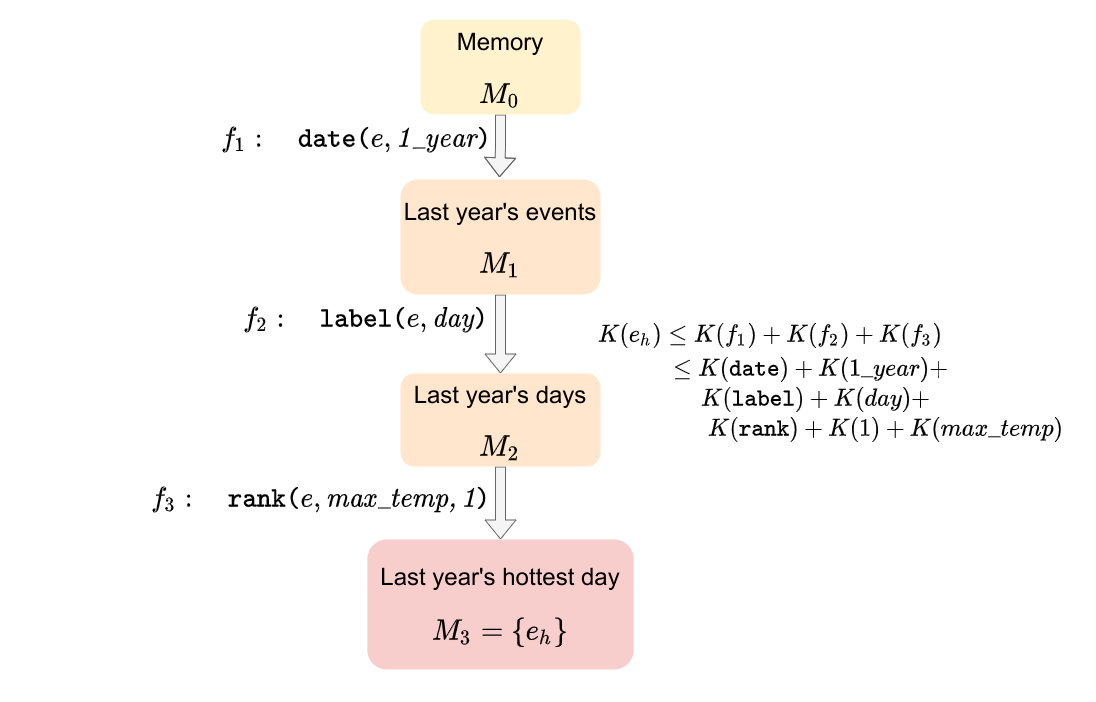
\includegraphics[width=.95\linewidth]{figures/filters}
    \caption{Retrieving an event through successive predicative
        filters. From the memory (yellow), successive filters select events satisfying the associated predicate (gray arrows). For example,
        filter $f_1$ selects events from last year, i.e. which satisfy the
        predicate $\mathtt{date}(event, 1\_year)$. In this case, successively
        applying filters $f_1$, $f_2$ and $f_3$ yields a unique event $e_h$, last
        year's hottest day. The complexity of this event can then be upper-bounded
        by the sum of the complexity of the three filters as they give an unambiguous way
        to describe the event within the memory.}
    \label{fig:filters}
\end{figure}

The rest of this article is organized as follows.
First, we briefly introduce
some relevant notions of Algorithmic Information Theory in subsection~\ref{sec:theory}. We then expose our contribution in subsections~\ref{sec:computing} with a formal definition of memorability. We present an implementation of these definitions with two smart-home examples in section~\ref{sec:results}. The results of these experiments are then presented and discussed. We explore other related works in subsection \ref{sec:related} and explore possible extensions of our work in subsection \ref{sec:future}.

\section{Theoretical Framework}
\label{sec:framework}

\subsection{Background}
\label{sec:theory}
Kolmogorov complexity formally quantifies the amount of information required
for the computation of a finite binary string\footnote{Though the definition
    holds for some infinite binary strings (think of the representation of the
    decimals of $\pi$), we restrict ourselves here to finite strings.} (or
any object represented by a finite binary
string)\cite{kolmogorov_three_1965,li_introduction_2008}. The complexity $K(s)$ of a (finite) binary string $s$ is the length in bits $L(p)$ of the shortest program $p$
which, if given as input to a universal Turing Machine $U$, outputs $s$.

\begin{equation}
    \label{eq:kolmo_def}
    K_{U}(s) = \min_{p}\left\{L(p)|U(p)=s\right\}\,.
\end{equation}

The first notable property of this definition is its universality: while the
choice of the Turing machine $U$ used for the computations appears in the
definition of Equation \ref{eq:kolmo_def}, all results hold, up to an additional
constant, if we change the machine. Think how any Turing-complete programming language can
be turned into any other language, using an interpreter or a compiler program. Since any
Turing machine $U'$ can be emulated by $U$ from a
finite program $p_{U}$, we have the following inequality:

\begin{equation}
    \label{eq:inequality_univ}
    K_{U'}(s) \le l(p_{u}) + K_{U}(s)\,.
\end{equation}

From this first result, we can then define complexity $K(s)$, based on the choice of a reference Turing machine, such that, for any other
machine $U$ taken from the set $\text{TM}$ of Turing machines:

\begin{equation}
    \forall U\in\text{TM}, \forall s, |K(s) - K_{u}(s)| \le C_{U}\,,
\end{equation}
where the additional constant $C_{U}$ does not depend on $s$.

Note that the notion of Kolmogorov complexity involves no requirement on the execution time of
programs; only their length in bits matters for the computation of
complexity. Though Kolmogorov complexity can be shown to be
incomputable~\cite{li_introduction_2008},
it can be approximated with
upper bounds by exhibiting a program outputting $s$.

Interestingly, Kolmogorov complexity matches the intuitive
notion and perception of complexity from a human standpoint. For instance, the
complexity of short binary strings evaluated in~\cite{delahaye_numerical_2012}
shows similar results to human perception of complex strings and patterns. More
recently,~\cite{murena_solving_2020} used Kolmogorov complexity to solve
analogies and showed results close to human expectations.

The bridge between Algorithmic Information Theory (AIT) and human perception of
complexity can be pushed farther thanks to the notions of simplicity and unexpectedness,
which are sometimes considered to be of uttermost importance in cognitive science~\cite
{chater_simplicity_2003}.
~\cite{dessalles_coincidences_2011} proposes a formal definition of the
unexpectedness $U(e)$ of an event, as the difference between an a-priori
expected causal complexity $K_{w}(e)$ and the actual observed complexity $K
    (e)$.

\begin{equation}
    \label{eq:unexpected} \textit{Unex}(e) = K_{w}(e) - K(e)\,.
\end{equation}

This result comes from the understanding that, while Kolmogorov complexity is
ideally computed using a Turing machine, it can be used as a proxy for modeling
information processing in the human brain, and thus can be used to define a notion of
simplicity or complexity of events. Hence, the term $K_w(e)$, which designates the causal complexity, models the cost of information that a hypothetical World Machine -- a Turing Machine modeling the person's understanding of the world -- would require to produce the observed outcome. This can be, for instance, the cost of different parameters in a physical model. As such, this quantity is highly dependent on the knowledge that the human subject has of its surrounding environment.

Definition \ref{eq:unexpected} allows to model phenomena
such as coincidences: imagine that you happen to run into someone in a park.
If this person has no particular link to you, the event will be quite
trivial: the complexity of describing this person will be equivalent to
distinguishing her from the global population, which is also roughly
equivalent to the (causal) complexity of describing the circumstances having brought this person to be in
that park as the same time as you. On the other hand, if you run into your best friend in
a park, as the complexity of describing your best friend is significantly
lower, the description complexity $K(e)$ drops while the causal complexity
$K_w(e)$ remains unchanged. This is why this latter  event appears unexpected. By contrast, if you knew beforehand that your best friend used to walk in this park, the causal complexity $K_w(e)$ would be significantly lower, hence reducing the surprise.

As~\cite{dessalles_coincidences_2011} suggests a link between unexpectedness and cognitive relevance, we propose to define the memorability of an event in a similar way. However, the proposed definition of unexpectedness, by introducing the hypothetical World Machine, results in an uncomputable metrics. Since we want to use this score in applications, we need a definition that is well-defined and computable in practice.
We therefore introduce the memorability $M(e)$ of an event as the absolute difference between its description complexity $K_d(e)$ and its expected description complexity $K_{exp}(e)$:

\begin{equation}
    \label{eq:memorability}
    M(e) = |K_{exp}(e) - K_d(e)|\,.
\end{equation}

Contrary to the definition of unexpectedness from Equation \ref{eq:unexpected}, we use an absolute value: we do so to acknowledge the fact that events more complex than expected can be memorable as well\footnote{In the original paper~\cite{dessalles2011coincidences}, exceptionally complex events are described by considering complexity itself as a way to describe the event: see ``the Pisa Tower effect''\cite{dessalles_pisa_nodate}}. In the next section, we define computational approximations for the description complexity $K_d$ and the expected complexity $K_{exp}$ of events.

\subsection{Defining and retrieving events}
\label{sec:computing}

%Computing the memorability of events begins with the introduction of formal definitions of events, how they are stored, how we can describe them and how these descriptions can be used to retrieve them.
We define \emph{events} as data points augmented with a \emph{label} indicating their nature (temperature event, failure event, addition/removal of a device) and a timestamp of occurrence. Formally:

\begin{equation}
    \label{eq:event}
    e = (l, t,\mathcal{D})\,,
\end{equation}
% ! response to Ada's remark: there is a hidden unique ID in the implementation, to distinguish between events; however this is not used to retrieve the event, as it is not a defining characteristics.
where $l$ is the label, $t$ the timestamp and $\mathcal{D}$ a vector of properties characterizing $e$: its duration, the maximum temperature reached, the sensor name, its position, etc. Labels can also be considered as classes of events, of which each event is a particular instance.

To model how humans are able to describe events by using qualifiers, we use \emph{predicates}: Boolean functions operating on events and, possibly, additional parameters: $\pi(e, a_1, a_2, \dots, a_n) \mapsto \{O,1\}$ is a predicate of arity $n$ operating on event $e$. In the rest of this paper, we will prefer the equivalent notation $\pi(e, k) \mapsto \{0,1\}$, where $k$ is a binary string encoding the sequence of arguments $a_1, \dots, a_n$. Using this notation, the predicate $\pi$ becomes a boolean function operating on $\mathbf{E} \times \{0,1\}^*$, where $\mathbf{E}$ denotes the set of all events:

\begin{equation}
    \label{eq:predicate}
    \pi : \begin{cases}
        \mathbf{E}\times \{0,1\}^{*} & \mapsto \{0,1\}    \\
        (e, k)                        & \mapsto \pi_{k}(e)\,.
    \end{cases}
\end{equation}

As an example of predicate, consider $\pi = \mathtt{year}$ and $k$ a string encoding the number $1$, thus
constructing the predicate $\mathtt{year(}e, 1\mathtt{)}$, which tells whether
the event $e$ occurred $1$ year ago. Another example would be the predicate $\pi = \mathtt{date}$, which can take as argument $k=\mathtt{year}::\mathtt{month}::\mathtt{day}$, and $\mathtt{date}(e, y, m, d)$ is true if and only if event $e$ occured at the specified date.

% ! response to Ada's remark: complexity computations don't consider time complexity, only program length. Indeed, using a FILO structure for the memory makes sense implementation-wise, but it does not affect the definitions of complexity and memorability. 
As events occur, they are stored in the  \emph{base memory} $M_0$. As they are not directly comparable, the memory $M_0$ can be considered as having the structure of an unordered set. We denote by $\mathcal{M}$ the set of all subsets of $M_0$. By extension, elements of $\mathcal{M}$, i.e. subsets of $M_0$, are also called \emph{memories}.

By applying a given predicate $\pi$ to all events contained in a memory $M \subseteq M_0$, and selecting only events satisfying $\pi$, one gets another memory $M_1 \subseteq M \subseteq M_0$. We call this operation a \emph{filter}:

\begin{equation}
    \label{eq:filter}
    f_{\pi, k}: \begin{cases}
        \mathcal{M} & \mapsto \mathcal{M}           \\
        M           & \mapsto \{e \in M | \pi_k(e) \}\,.
    \end{cases}
\end{equation}

For instance, using the same $\pi = \mathtt{year}$ and $k=1$ as above, we can
build the filter $f_{\pi, k} = \mathtt{last\_{}year}$, which selects all events
that occurred last year.

As the output of a filter applied to a memory $M$ is another memory
object $M' \subseteq M$, we can compose filter
functions. A sequence of such filters is called a \emph{retrieval path}

\begin{equation}
    \label{eq:ret_def}
    p = (f_{\pi_{1}, k_{1}}, \dots, f_{\pi_{n}, k_{n}})\,.
\end{equation}

By definition
$p(M) = f_{\pi_{n}, k_{n}}(\dots(f_{\pi_{1}, k_{1}}(M)))$.
In case the result of the operation $p(M)$ contains a single element
$e$, we say that the path $p$ \emph{retrieves} the element $e$ from $M$, and write
$p(M) = e$. In the example shown in Figure \ref{fig:filters}, the three filters $f_1, f_2, f_3$ form a retrieval path retrieving the event ``last year's hottest day'' from the base memory $M_0$.

\subsection{Description complexity of events}

As presented in sec. \ref{sec:theory}, we are interested in computing an approximation of the description complexity of an event $e$. From the above definitions, if there is a path $p$ retrieving $e$ from the base memory $M_0$, i.e. $p(M_0) = e$, this path provides a possible unambiguous description for $e$. We define the description complexity of $e$ as the minimum complexity of a path $p$ retrieving $e$ from the base memory $M_0$.

\begin{equation}
    \label{eq:k_desc}
    K_d(e) = \min_{p \in P_\infty} \{L(p) | p(M_0) = e\}\,,
\end{equation}
where the bit-length $L(p)$ of a retrieval path is defined as the number of bits of a string encoding the path. If we limit ourselves to prefix-free strings encoding predicates and arguments, the total bit length is given by:

\begin{align}
    \label{eq:bit_lenght_p}
    L(p) & = L((f_{\pi_1,k_1}, \dots, f_{\pi_n, k_n}))     \\
         & = L(\pi_1) + L(k_1) + \dots + L(\pi_n) + L(k_n)\,,
\end{align}
where $L(\pi_i)$ and $L(k_i)$ denote the length, in bits, required to express the predicate's concept and program, respectively. This length may vary depending of the encoding choice, see Section \ref{sec:results} for an example.

By considering only a finite number of possible predicates $\pi$ and arguments $k$, and a maximum path length, we can construct a finite set $P$ of possible retrieval paths. By limiting the search over this set, we get an upper bound of description complexity, and use this upper bound as an approximation:

\begin{equation}
    \label{eq:approx_k_desc}
    K_d(e) \leq \min_{p \in P \land p(M_0) = e} L(p) = \min_{p \in P \land p(M_0)=e} \sum_{f_{\pi, k} \in p} L(\pi) + L(k)\,.
\end{equation}

The approximation of description complexity from Equation \ref{eq:approx_k_desc} allows for
a direct implementation, which is shown in Algorithm \ref{alg:complex_iter}. This
algorithm operates iteratively: starting from the base memory $M_0$
(line 1), we apply all possible predicate concepts $\pi$ from a given finite set
$\Pi$ and programs $k$ (lines 6-7), up to a given length $\mathtt
{max\_len}$ bits, and apply them: $M' = f_{\pi, k}(M)$ (line 12). We then store
the pairs $(M', \mathtt{len(}\pi, k\mathtt{)})$ in an array $\mathtt{future_
{explore}}$. At the end of the iteration, the results of the filters become the
memories which will be explored during the next iteration(lines 21--23). Each
pass thus explores retrieval paths of increasing length. When a singleton memory
is reached, the complexity of its unique element is upper-bounded with the
length of the corresponding retrieval path (line 14).

\begin{algorithm}
    $\mathtt{current_{explore}} \leftarrow [(\mathcal{M}, 0)]$ \;
    $\mathtt{future_{explore} \leftarrow} [\;]$ \;
    $\mathtt{pass} \leftarrow 0$ \;
    $\mathtt{K(e)} \leftarrow +\infty$ \;
    \While{$\mathtt{current_{explore}} \neq [\;]$ \textbf{and} $\mathtt{pass} < \mathtt{max\_pass}$}{
    \For{$(\mathtt{M_{prev}}, \mathtt{K_{prev}}) \in \mathtt{current_{explore}}$}{
    \For{$\pi \in \mathcal{P}$}{
    \For{$\mathtt{k \in \{0,1\}^{*}}$}{
    $\mathtt{K_{current}} \leftarrow L(\pi) + L(k) + \mathtt{K_{prev}}$ \;
    \If{$\mathtt{K_{current}} > \mathtt{max_{complex}}$}{
        \textbf{break} \;
    }
    $\mathtt{M'} \leftarrow f_{\pi,k}(\mathtt{M_{prev}})$ \;
    \eIf{$\mathtt{M'} = \mathtt{\{e\}}$}{
        $\mathtt{K(e) \leftarrow \min(K(e), K_{current})}$ \;
    }{
        $\mathtt{future_{explore}.append((M', K_{current}))}$\;
    }
    }
    }
    }
    $\mathtt{current_{explore}} \leftarrow \mathtt{future_{explore}}$ \;
    $\mathtt{future_{explore}} \leftarrow [\;]$ \;
    $\texttt{pass} \leftarrow \mathtt{pass} + 1$\;
    }
    \caption{Iterative computation of the approximate complexity}
    \label{alg:complex_iter}
\end{algorithm}
% ! response to Ada's comment: yes, this works well ;-) It is even implemented in the code. However, given that time complexity does not impact the definitions of complexity, I decided to present the simplest program, not the most optimized, for the sake of clarity.

\subsection{Computing Memorability}
As stated in Equation \ref{eq:memorability}, we define memorability $M(e)$ as the absolute difference between the description complexity of an event and its expected value. As we've just defined $K_d(e)$ and provided an approximation in Equation \ref{eq:approx_k_desc}, we now focus on defining the \emph{expected} description complexity of an event, $K_{exp}(e)$ that appears in Equation \ref{eq:memorability}.

$K_{exp}(e)$ evaluates the complexity that the user, or the system, would expect for the occurrence of event $e$ to have, based on their previous knowledge. In our framework, this prior knowledge consists of the base memory $M_0$. The expected complexity of the event $e$ can be computed with a simple first-order approximation, i.e. estimating the average complexity of ``similar events'' over the base memory $M_0$.

Still, there is a difficulty in defining what
should be considered \emph{similar} events. Given that we deal with non comparable events, we may define the notion of similarity by referring once again to \emph{predicates}. For a given event $e$ and a given predicate $\pi_k$, we define a $\pi_k$-neighborhood of $e$ as the set $N_{\pi, k}(e)$ of all other events satisfying $\pi_k$.

\begin{equation}
    \label{eq:similar}
    N_{\pi, k}(e) = \{e'\in M_0, (e' \neq e) \wedge \pi_k(e')\}
\end{equation}

Now, when considering, for all possible predicates $\pi_k$, the corresponding
neighborhoods $N_{\pi, k}(e)$, with the convention that $N_{\pi, k}(e) = \emptyset$
if $e$ does not satisfy $\pi_k$, we can compute an average expected complexity for $e$, by summing the complexity of events in all neighborhoods of $e$ and dividing the total by the number of events in the neighborhoods:

\begin{equation}
    \label{eq:expected}
    K_{exp}(e) = \frac{
    \sum_{\pi, k} \sum_{e' \in N_{\pi, k}(e)} K_d(e')
    }{
    \sum_{\pi, k} |N_{\pi, k}(e)|
    }\,.
\end{equation}

This definition is consistent with the intuitive idea that more similar events should weigh more in the computation. Indeed, if $e'$
is very similar to $e$, it will appear in many neighborhoods, since it
satisfies most of the predicates that $e$ satisfies. Therefore, it will
be present in more terms in Equation \ref{eq:expected}, and will weigh more in
the final result.
% ! response to Ada's comment: Yes, it is. If a point belongs to many neighbourhoods, with many points in each, it will be hard to distinguish from the other points. So, its expected complexity is hard. Think, for instance, of the expected complexity for a human being: it will be roughly log2(7000000000) bits, for a randomly picked person. If this person is known to you, it will be simpler to describe her. 

This metrics solves the different problems exposed in the introduction: by using a universal measure for complexity, bits, it allows to compare values from different dimensions. For instance, it solves the dilemma of recent events: is a big event a long time ago more memorable than a smaller one that occurred only a few minutes ago? With our approach to complexity, each one of these dimensions will scale logarithmically, with the bit length of the required predicate parameters. The balance between them depends on the subjectivity of the system, which is encoded in the intrinsic complexity of predicates for magnitude and dimension. 

\subsection{Defining relative memorability for abduction}
% TODO : see ada's comment for this part
Abductive inference builds upon the computation
of the memorability score. \emph{Knowing} that we want to find a cause $c$
for an observed effect $e$, we try to find the most remarkable event in
memory that is related to $e$. While our ``memorability'' score identifies remarkable past events, it does not take into account their relatedness to $e$.

The knowledge attached to the occurrence of $e$ can be integrated into the description complexity definition by using conditional complexity $K_d(c | e)$: The information contained in $e$ is considered as given, and therefore as ``free'' in terms of complexity. For instance, when looking for a cause of
an anomaly in the living-room, other anomalies occurring in the same
living-room will be simpler, as the location ``living-room'' is already known
from the observation of the current anomaly.

Formally, we now consider that knowledge of the effect is given. This consists, for instance, of appending a description of effect $e$  to all programs $k$:
$\pi_{e::k}(c)$, where $::$ is the \emph{append} operation. The set of paths obtained with such predicates is noted $P^\infty_e$. This \emph{append} operation is free in terms of bit-length in the computation of complexity, since the effect event $e$ is an input of the problem. Therefore, we have $L'(\pi_{k::e}) = L(\pi_k) = L(\pi) + L(k)$. We get a definition for the conditional description complexity:

\begin{align}
    \label{eq:abd_k}
    K_d(c | e) & = \min_{p \in P^\infty_e} \{L'(p), \quad p(M_0)=c \}\,,                                                \\
               & = \min_{p \in P^\infty_e} \left\{\sum_{f_{\pi, k::e} \in p} L(\pi) + L(k), \quad p(M_0) = c\right\}\,.
\end{align}

This new conditional description complexity translates the additional information provided to the
system when answering a user's request. It can then be averaged over similar events to compute the expected conditional description complexity, $K_{exp}(c|e)$. From this, we come to the definition of the \emph{conditional memorability}, which measures how memorable an event $c$ turns out to be in the context of the occurrence of another event $e$:

\begin{equation}
    \label{eq:cond_mem}
    M(c|e) = |K_{exp}(c|e) - K_d(c|e)|\,.
\end{equation}

Conditional memorability encapsulates the idea
presented as the motivation of this paper: when confronted with a surprising
situation, and in the absence of any other source of information, events that appear more memorable than others with regards to the target event will be selected as potential causes. As such, our conditional memorability score provides a ranking that can be used for abductive inference.



\section{Experiments}
\label{sec:results}
\subsection{Setup}
\label{sec:setup}

We design two different setups to test our approach. Both are inspired from smart home use cases.  This choice of
configuration is motivated by the challenges posed by smart homes for abductive
inference: i) as the number of connected devices increases, more events are
recorded, making the detection of memorable events more important; ii) smart
homes are prone to experience atypical situations, highly dependent on the context,
for which pre-established relations might fail to find good abduction
candidates. Our choice was also motivated by
the existence of previous work~\cite{lalanda_self-aware_2017} involving smart home simulations capable of quickly generating data from which we could extract events and test our methods.

% \subsubsection{Scenario 0}
% First, we study a simple situation where the frequency of an event, and not its magnitude, makes it remarkable. Consider a delivery truck servicing a store. One apparition of this truck in the street is registered as an event. Over a period of 200 days, on most days, the truck appears at most once per day, to deliver the store. However, on one particular day, the truck appears over a dozen times in the street! The sudden high frequency of appearance makes observations of the truck on that particular day more memorable, while remaining individually the same.

\subsubsection{The ``TV'' scenario}
In this setup, we aim to reproduce the example mentioned in Section \ref{sec:introduction}: installing and using for the first time a brand new smart TV causes unpredictable effects on the light of the room where the TV is located. Faced with this situation, history-based approaches fail to identify the right hypothesis as there is no previous data for the new TV. To play this situation, we created a set of events covering a period of 100 days, corresponding to the past knowledge of the house. Two kinds of events are recorded: ``TV event'', corresponding to TV use (old and new); and luminosity events, describing the luminosity of the room at a given time. Low lights occur at night, and can occasionally occur during daytime (for instance if the blinds are down). On the 100\textsuperscript{th} day, a ``TV event'' is recorded with a different ``device'' characteristic: it corresponds to the first usage of the new smart TV. Shortly after, the light dims, which is recorded in a ``light'' event.

\subsubsection{The ``temperature'' scenario}
We consider an experimental smart home setup with various sensors, which we simulate over a period of time. The smart home simulation data is then processed to identify some predefined events (such as abnormal temperatures).
To carry out the simulation, we used the iCasa smart home simulator platform~\cite{lalanda_self-aware_2017} 
to which we added custom modules. iCasa
allows the simulation of autonomic systems that can handle internal communications,
the possible insertion of new components at runtime, or the deletion or modification of existing
components. We used a basic scenario consisting of a house with four rooms,
a single user, and an outdoor zone. All four rooms are equipped
with a temperature control system in charge of heaters (see Figure.
\ref{fig:view}).

\begin{figure}[!ht]
    \centering
    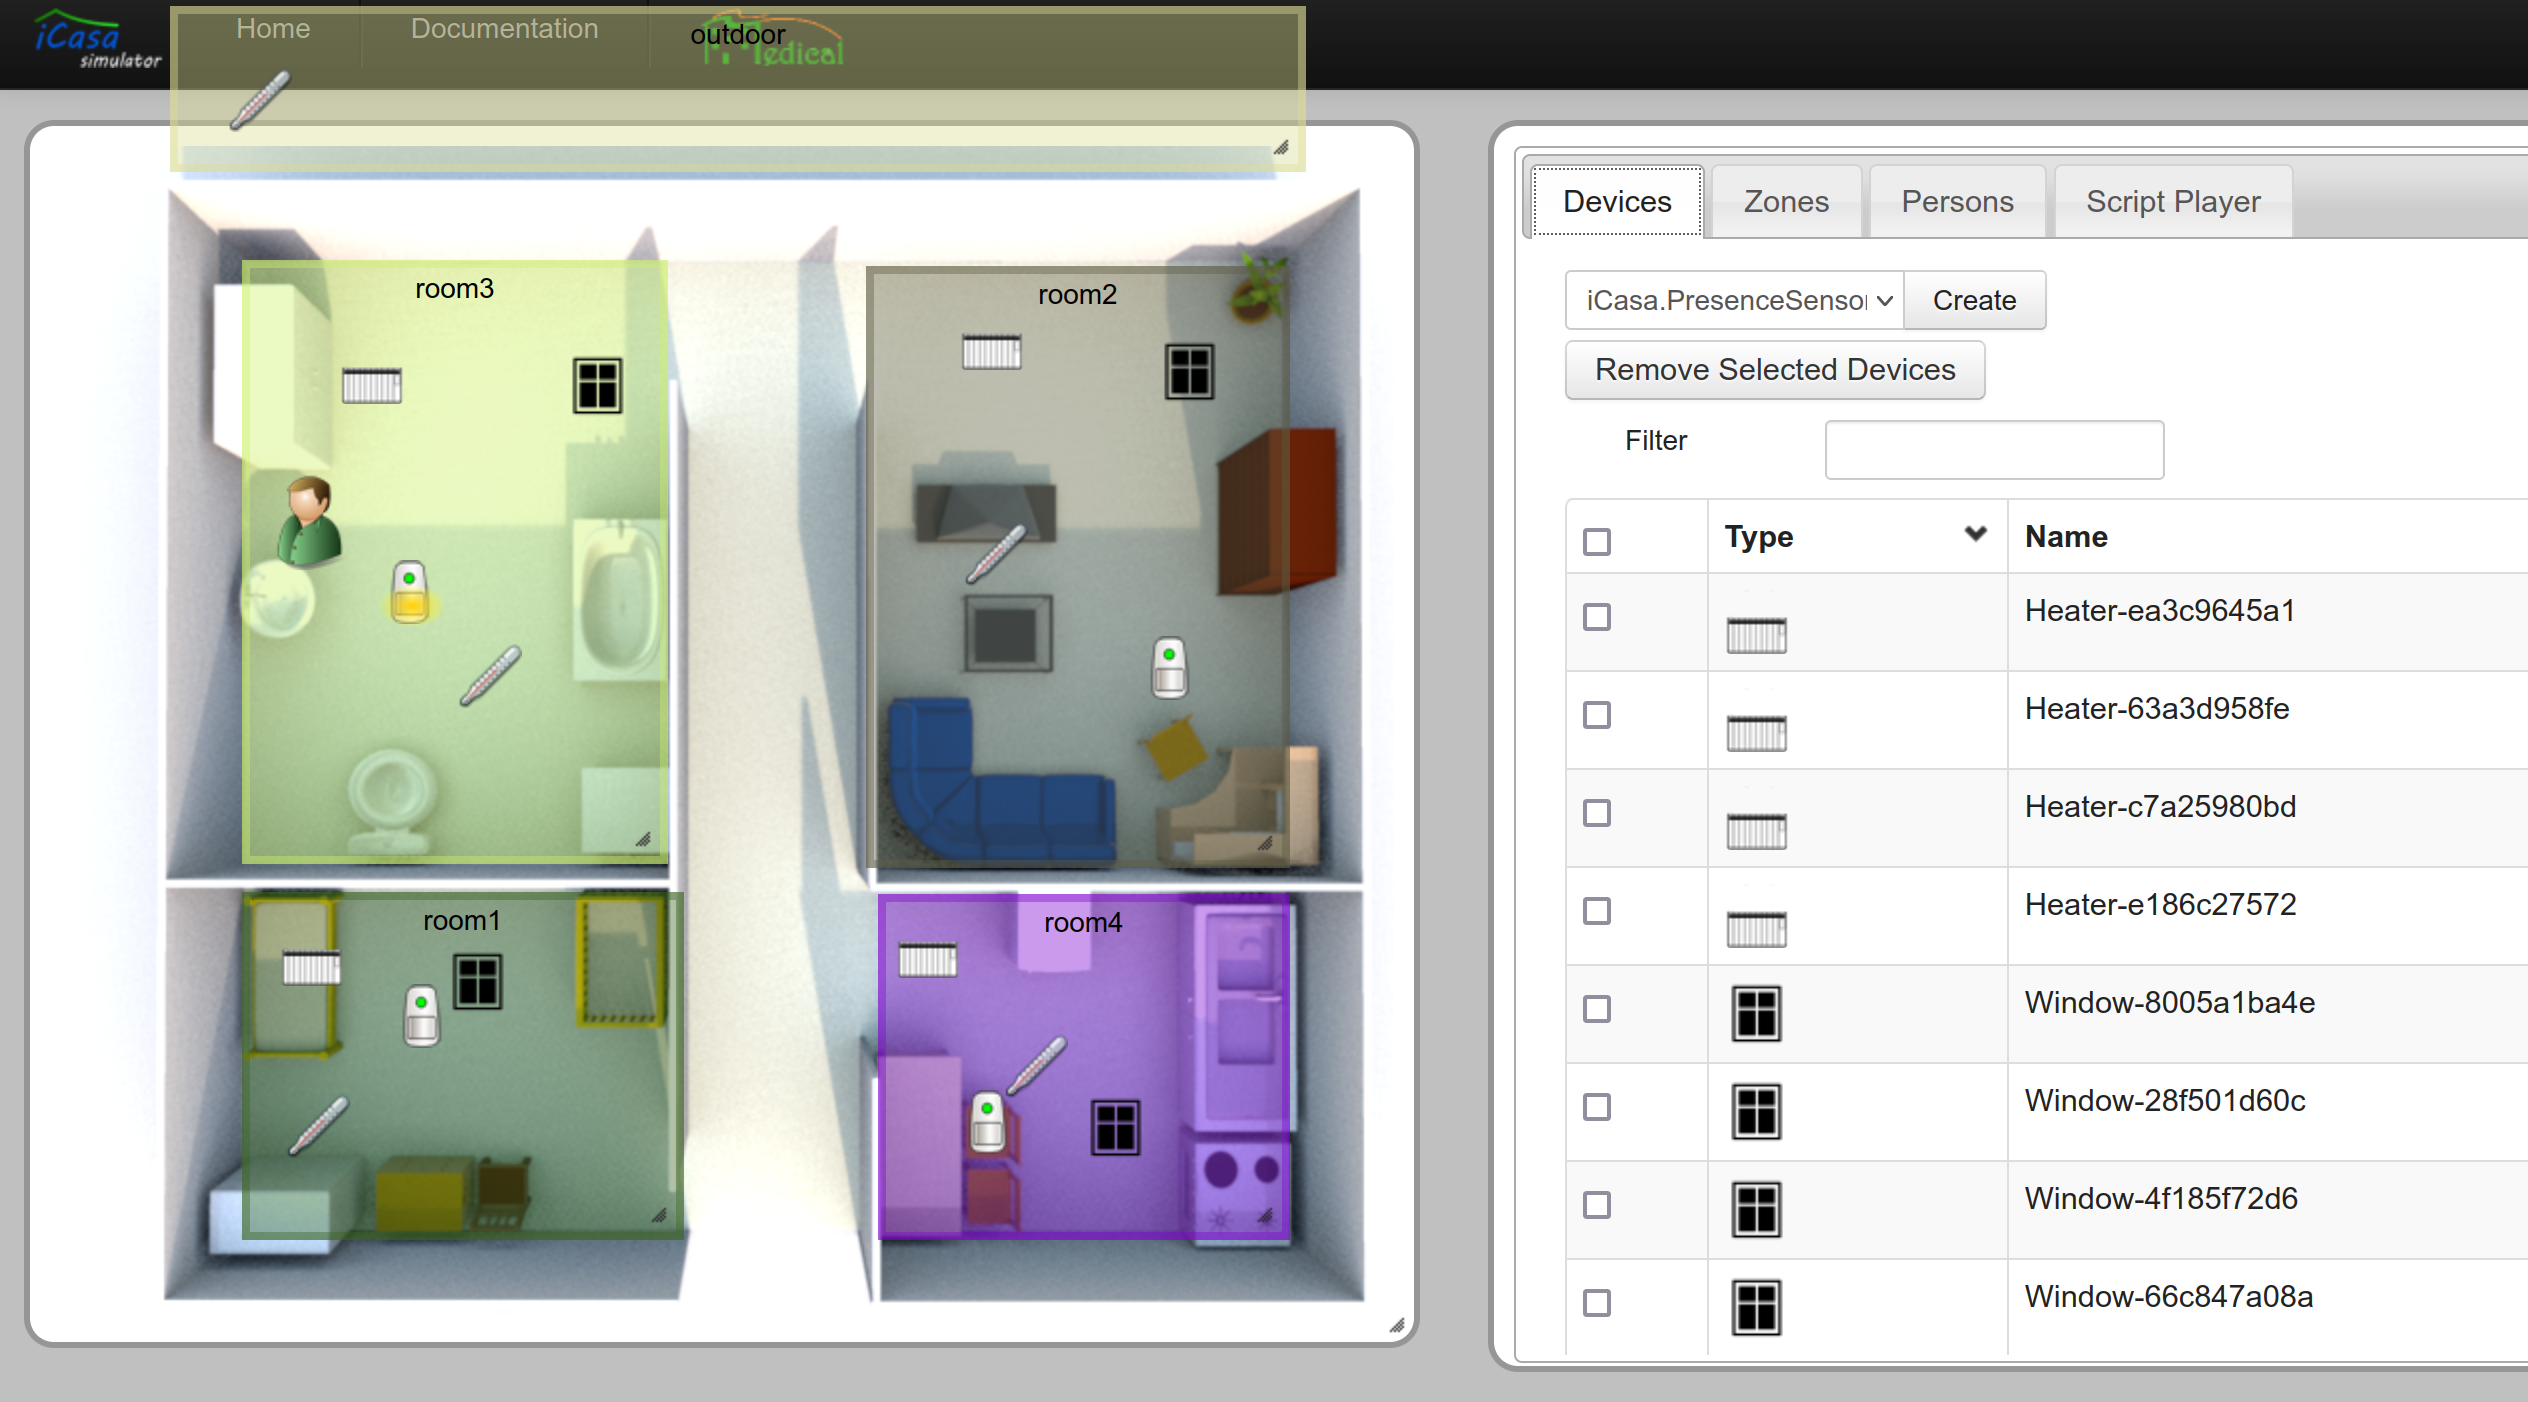
\includegraphics[width=.8\linewidth]{figures/icasa_interface.png}
    \caption{View of the simulator's web interface provided by iCasa. The four
        rooms are visible, with their equipment and the user.}
    \label{fig:view}
\end{figure}

Based on this, we implemented a scenario spanning over 420 days, and
comprising a daily cycle of outdoor weather (temperature and sunlight) fluctuations, as well
as user movements. All these daily changes create non-noticeable events,
serving as a background for our experiments. To produce outstanding
events, we randomly generated about twenty special events, spanning over the whole
duration of the simulation. These outstanding events were of the following kinds:

\begin{itemize}
    \item Unusual weather: the outdoor conditions are set to unusually high or
          low temperatures.
    \item Heater failures: heaters may break down, making them turn off regardless
          of the command they receive.
          % \item User's absence: the user goes out of the building for an extended
          %       period of time.
    \item Device removal/addition: a device is removed, or another one is added
          to the system.
\end{itemize}


Values observed from all devices and zones were sampled throughout
the simulation. The resulting data (figure
\ref{fig:ts_example}) was then used as a basis for our experiments.
We then process the time series data to identify and characterize events.
Since the ways events are detected is not the focus of our present work (see Section.
\ref{sec:related}), we perform event detection merely based on threshold comparison, e.g. an temperature event is created if temperature measure are above a given threshold for more than a certain amount of time.

\begin{figure}[!ht]
    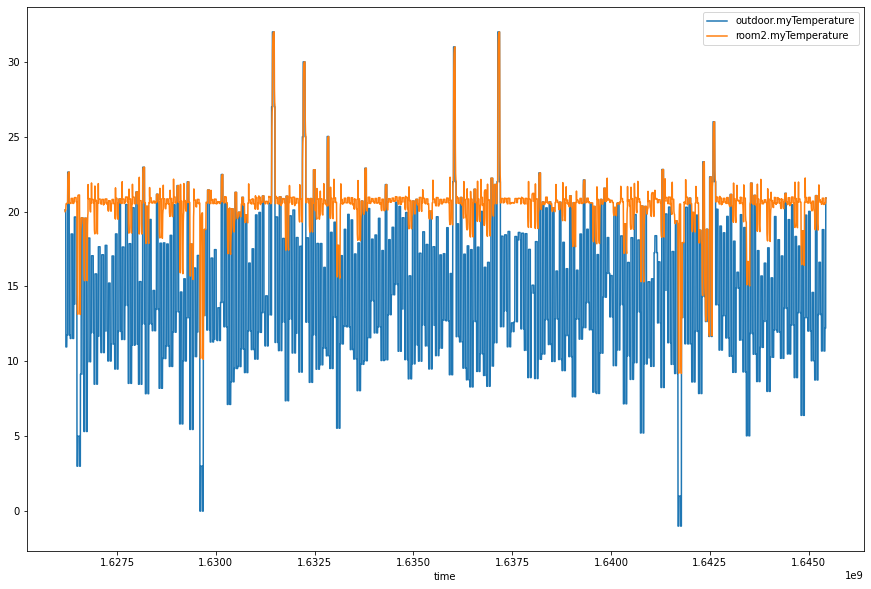
\includegraphics[width=\linewidth]{figures/ts_example}
    \caption{Time series data from the simulation: outdoor temperature (red) and
        controller temperature of a room (blue). To be used in our framework, these time series data are
        processed by a simple threshold-based event detection.}
    \label{fig:ts_example}
\end{figure}


\subsection{Implementing the complexity computation}

We implemented the computation of both the description complexity and the memorability score into a Python object, called the \texttt{SurpriseAbductionModule}. Apart from the base memory of events $M_0$, this module contains a set of predefined predicates $\Pi$ to characterize events. For instance, for scenario 2, the predicates we use are the following:
\begin{itemize}
    \item $\mathtt{label(e, k)}$: whether the event $e$ has the $k^{th}$ most frequent label (meaning that frequent labels are simpler to express than rare ones)\footnote{In case some labels have the same frequency, an arbitrary rank is used among them. However, given the unlikeliness of this occurrence, the impact on complexity is insignificant (this case did not occur in our test examples with a few hundreds events).}. In case some labels have the same frequency, a rank is assigned 
    \item $\mathtt{rank(e, r, a)}$: whether the event $e$ is ranked $r^{th}$ for characteristic $a$, where characteristics are encoded by their frequency (again, common characteristics are the simplest ones)
    \item $\mathtt{day(e, k)}$: whether the event $e$ occurred $k$ days ago.
          % \item $\mathtt{randomChoice(e, k)}$: whether the event $e$ id matches the program $k$, which can be regarded as a random seed.
    \item $\mathtt{month(e, k)}$: whether the event $e$ occured $k$ months ago.
    \item $\mathtt{location(e, k)}$: whether the event $e$ occurred in zone
          $k$.
\end{itemize}

% Similar predicates were used for scenario 1. However, to show the impact of allowing random selection of events, we added a \texttt{RandomPick} predicate, which is true if the id of the event matches a random program seed $k$. As it could be argued that in some cases, randomly selecting an event is not possible, we decided to implement this predicate in only one scenario.

% with the notable exception of the addition of a \texttt{RandomPick} predicate, which is true if the id of the event matches a random program seed $k$. Using this predicate and the associated filter in only one of the two illustrative examples shows the importance of allowing random selection in the complexity computation. Furthermore, it could be argued that in some case, random selection of an event is not possible.

The description length $L(\pi, k)$ of a predicate $\pi_k$ is computed as follows: since the set of predicates is finite and known, $L(\pi) = \log_2(|\Pi|)$ bits are enough to describe the predicate concept $\pi$\footnote{This approach gives an equal complexity to all predicate concepts. Though this choice may be questionable when using many concepts, as humans do, we we used this simplification as our examples rely on few predicates.}. To encode the argument $k$ of the predicate, we used the widely used prefix-free Elias delta code~\cite{elias_universal_1975}, which requires $L(k) = \log_2(k) + 2 \log_2(\log_2(k)+1) + 1]$ bits. The total cost of describing $\pi_{k}$ therefore is

\begin{equation}
    \label{eq:pred_cost}
    L(\pi, k) = \log_2(|\Pi|) + \log_2(k) + 2 \log_2(\log_2(k) + 1) + 1\,.
\end{equation}

With a straightforward implementation of memory, predicates and filters, we could run Algorithm \ref{alg:complex_iter}. However, it took too
long to be usable in realistic scenarios with hundreds or thousands of events to
consider. In order to facilitate and speed up computations, we implemented
the following improvements:
\begin{itemize}
    \item The memory object was augmented with various built-in rankings, allowing
          for faster operations during filtering. For instance, since the memory
          object keeps a mapping from timestamp to events one can perform a quick
          filtering by date without having to loop over all stored elements. This convenient mapping,
          however, is not directly used to retrieve events by their date of occurrence, so as to
          preserve the theoretical model of memory as an unordered set, as presented in
          section \ref{sec:computing}.

    \item Each of these predicates holds the property that, in addition to
          \texttt{True} and \texttt{False}, they can return another value,
          \texttt{None}, which is theoretically treated as \texttt{False} but carries
          the additional information that this predicate concept will also be false for
          any other element of the memory for any subsequent program $k$. This allows to
          effectively break the innermost loop in alg. \ref{alg:complex_iter}.

    \item Some of the filters, for instance the date and rank filters, were
          hard-written. Events can be selected from these precomputed mappings over the memory objects
          rather than by testing a predicate over all memory elements.
\end{itemize}

Our code is written in Python. Examples are presented in the form of Jupyter Notebooks, which allow to quickly reproduce our results and figures. All code is available on our Github: \url{https://github.com/EtienneHouze/memorability_code}. Figures from the code are interactive: hovering the mouse above points displays the iD of the event, as well as the predicates used in the optimal retrieval path.


\subsection{Results}
\label{sec:example}

% \subsubsection{The ``Truck'' scenario (scenario 0)}
% For this scenario, a random sampling of events resulted in 57 seeings of the delivery truck in the street, 21 of them occurring in the same ``remarkable'' day. The results of the complexity computations of our methods are displayed in Figure \ref{fig:freq_complex}. They show that events from the ``remarkable'' day are more complex than other appearances of the delivery truck. This happens because the amount of information required to describe an event from that particular day is higher: it requires additional temporal information, such as the hour and minutes of appearance. As such, our method shows its potential in defining memorability not only in terms of magnitude of events, but also in terms of their frequency of apparition.

% \begin{figure}[!ht]
%     \centering
%     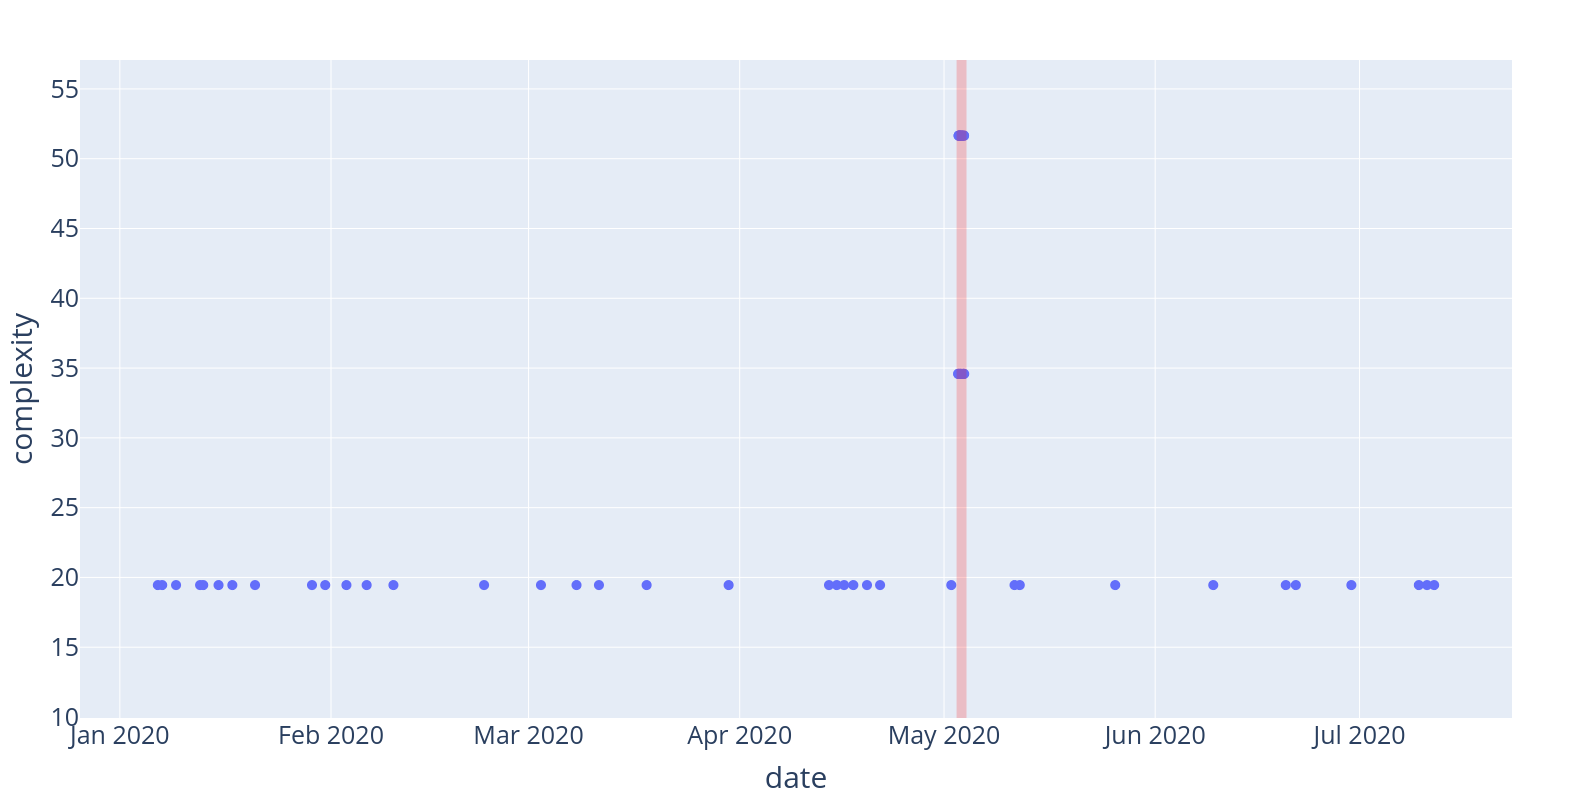
\includegraphics[width=.9\linewidth]{figures/complexity_frequency.png}
%     \caption{Complexity of the truck events in Scenario 0. Observations from the ``remarkable'' day, in red, stand out as more complex than the rest.}
%     \label{fig:freq_complex}
% \end{figure}

\subsubsection{The ``TV'' scenario}
\paragraph{Memorability}

The computation of the description complexity measure for the 2500 recorded events took around 90 seconds using an i7-8565u-equipped laptop. The resulting memorability scores are shown in Figure \ref{fig:scenar1_complexity}. We can observe that, on average, recent events are given a higher score: this reflects the cost of designating an event by the time elapsed since its occurrence. Furthermore, we can see that some light events, in blue, are more memorable than the main sequence. These events correspond to either events that occurred simultaneously to TV events, in pink: as they are simultaneous to another event, they require additional information to be singled out, temporal information not being enough. Thus, they appear as ``surprisingly'' more complex than the rest of their king, hence more memorable. 


Some light events also appear more memorable than the rest: they are events when light was surprisingly low given the hour and therefore are easier to retrieve. While these general observations are consistent with an a-priori intuition, the results are dependent of the choice of predicates used for the computation. See section \ref{sec:discussion} for a discussion on this dependence.


\begin{figure}[!ht]
    \centering
    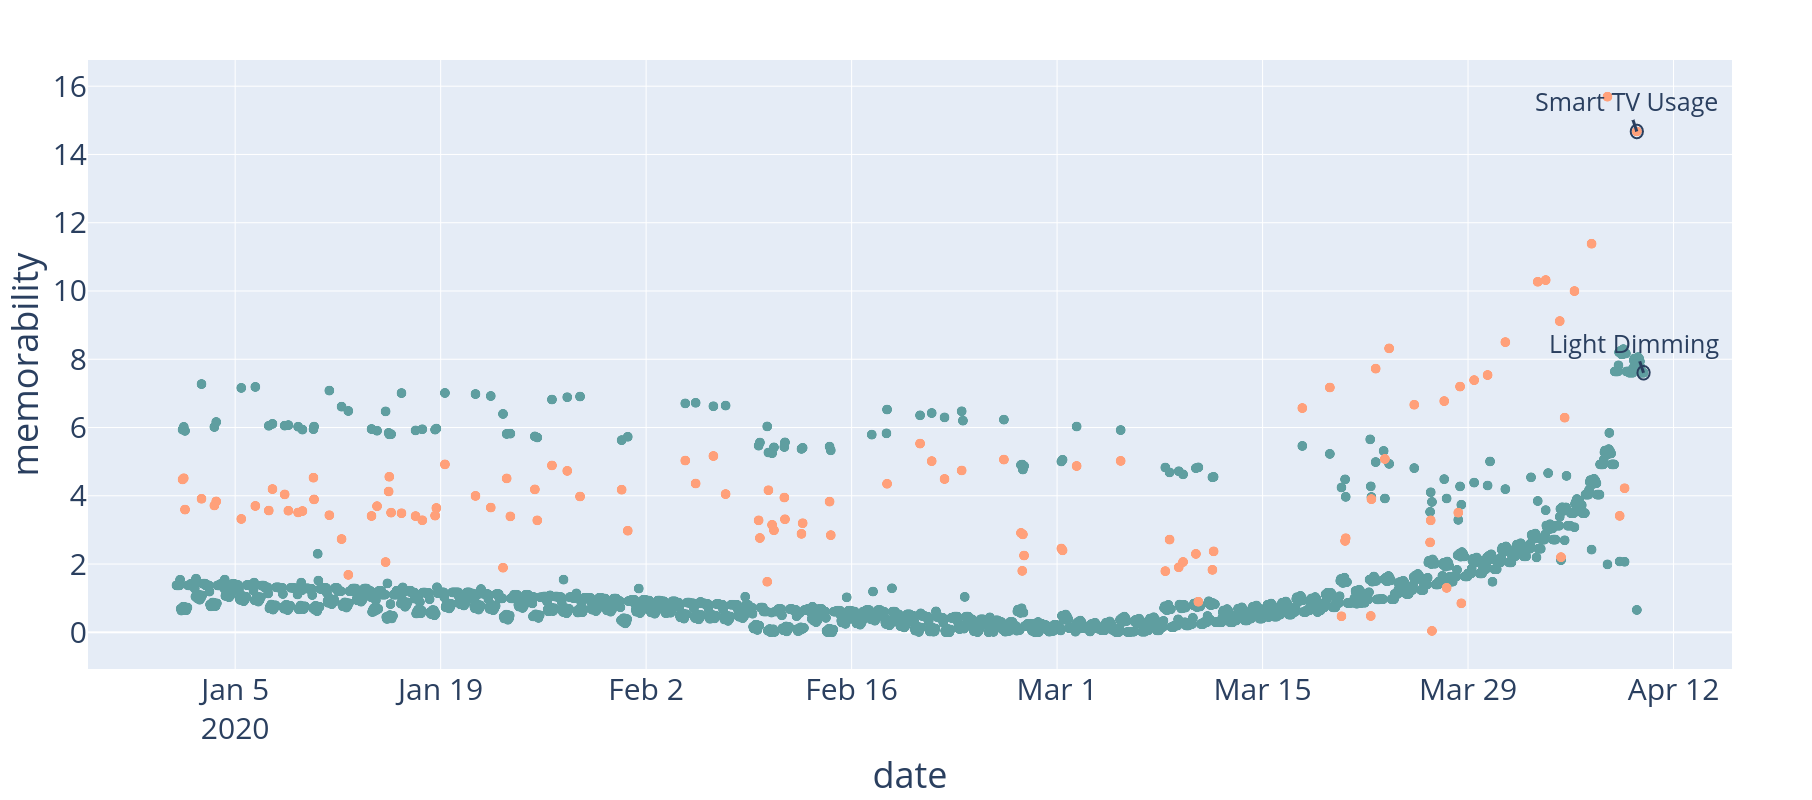
\includegraphics[width=.9\linewidth]{figures/memo_scenar_1.png}
    \caption{TV scenario. Computed memorability for events. Luminosity events are shown in blue, TV events in pink. The two circled events are the ones mentioned in the scenario.}
    \label{fig:scenar1_complexity}
\end{figure}

\paragraph{Abduction}
To show the potential application to abductive inference, we use our approach for abduction in the first scenario, to see if memorability alone can find the brand new TV to be a reasonable cause for the sudden light dimming.

The result of our algorithm is given in Table \ref{tab:abduction_res}: the system correctly identifies the new TV as being the cause. The reason for this choice is that, since the smart TV's device ID is unique among all other events of type ``TV'', its description complexity stands out as being significantly lower than the others, and therefore entails a high memorability score. While our method does not guarantee the correctness of the hypothesis (in fact, abductive reasoning cannot offer such a guarantee \cite{magnani_abduction_2011}), it provides an alternate hypothesis which corresponds to what a human may have suspected in this case where previous knowledge is unavailable.

\begin{table}
    \centering
    \begin{tabular}{l|c|c}
        Event Id & Description                   & Relative memorability (bits) \\
        \hline
        2513     & Use of smart TV               & 16.76                        \\
        2427     & Last use of the old TV        & 14.81                        \\
        2411     & Second-last use of the old TV & 11.21
    \end{tabular}
    \caption{TV Scenario. Output of the memorability-based abduction module: top 3 events for the relative memorability metrics.}
    \label{tab:abduction_res}
\end{table}

\subsubsection{The ``temperature'' scenario}
% \paragraph{Memorability}

For this scenario, 578 events were recorded from the setup described in Subsection \ref{sec:setup}. THe computation of the memorability and complexity scores took around 30 seconds on a commercial laptop equipped with an i7-8565u CPU. Four loops of Algorithm \ref{alg:complex_iter} where required (as additional loops did not improve scores).

Similar to the previous scenario, the general trend of events appears as a time-dependent logarithmic score for most events: this corresponds to events for which the simplest retrieval path consists of describing the elapsed duration since their occurrence using the \texttt{day} predicate. As such, it appears that most days are considered ``usual'' by our memorability score. This effect produces the main logarithmic sequence of blue dots. On the other hand, some events stand out in terms of
complexity: some appear simpler, as they can be distinguished by using their
rank along some axis (``the hottest day'', ``the second coldest day''), or the rare occurrence of their kind (``the only recorded failure of the heater'').

\begin{figure}[!ht]
    \centering
    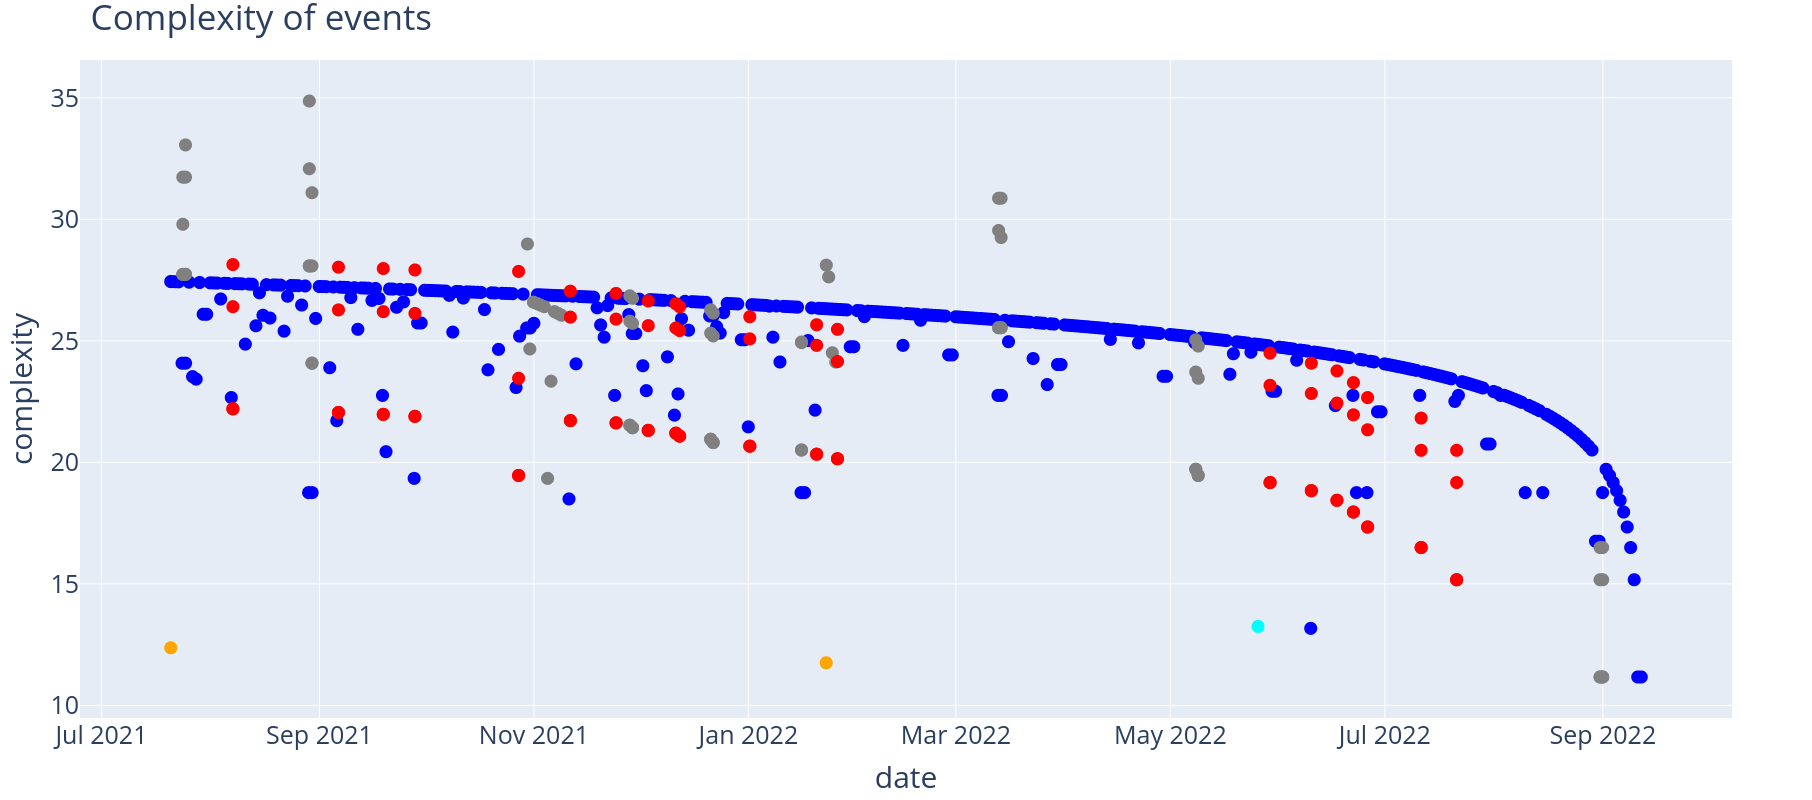
\includegraphics[width=.9\linewidth]{figures/complexity_scenar_2.png}
    \caption{Temperature scenario. Description complexities of events with retrieval paths of
        length at most 4. Events of type ``day'' (blue), ``hot'' (red), ``cold''
        (gray), ``device removal''(orange) and ``device addition'' (cyan) are shown.}
    \label{fig:computed_cplx}
\end{figure}

The ``memorability score'' is shown in Figure \ref{fig:result1}. Similar to what happened with the description complexity score, most events appear with a low memorability: this corresponds mostly to events from the ``main sequence'' from Figure. \ref{fig:computed_cplx}. On the other hand, some events stand out : for instance events 20 and 329, which are respectively the hottest and coldest days recorded, or event 183 which correspond to the rare type \emph{device\_removal}.
Since our memorability measure treats unusually complex or unusually simple events the
same way (from the absolute value operation in Equation \ref{eq:unexpected}), we
observe that some events are memorable due to their context only. For instance,
the group to which event 149 belongs appears more complex than expected: the same event occurring simultaneously in all four rooms of the house make each instance harder to discern.
Table \ref{tab:paths} illustrates this by exhibiting the retrieval paths used for complexity computation for these events.

\begin{table}
    \centering
    \begin{tabular}{c|c|c}
        Event iD & Event Type    & Retrieval Path                             \\
        \hline
        20       & day           & Label("day"), AxisRank(0, "max\_temp")     \\
        329      & day           & Label("day"), AxisRank(0, "min\_temp")     \\
        183      & deviceRemoval & Label("deviceRemoval"), Day(0)             \\
        149      & cold          & Label("cold"), Day(2), Device("thermo\_2") \\
    \end{tabular}
    \caption{Temperature scenario. Selected events with their shortest retrieval path.}
    \label{tab:paths}
\end{table}

\begin{figure}[!ht]
    \centering
    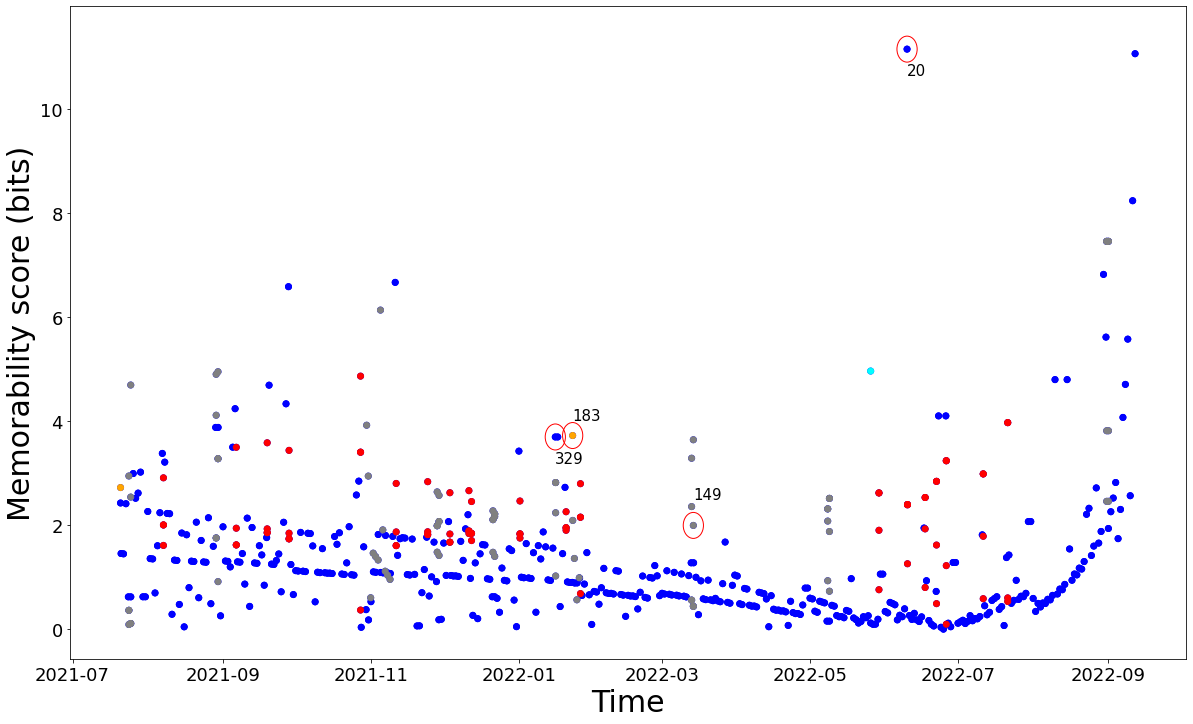
\includegraphics[width=.9\linewidth]{figures/memo_scenar_2.png}
    \caption{Temperature scenario. Memorability score for events in memory. Events mentioned in the text are highlighted.}
    \label{fig:result1}
\end{figure}

% todo: reproduction of the ROC curve. see with the python code
Given that we generated the data used for this experiment, it is possible to
flag all perturbation events apart from the usual daily events and evaluate how a
detection based on the ``memorability'' score would perform in distinguishing these
events. The result is presented as a ROC curve in Figure \ref{fig:roc}, obtained by varying the memorability threshold. This shows the memorability score's performance as a classifying tool for ``out-of-the norm'' events. In this example, memorability alone correctly identified 18 manually generated events with only 5 false-positives. While the direct application of memorability for classification or event detection is not within the scope of this paper (see Section \ref{sec:related} for complexity-based detection), this first result is on par with the motivation of memorability being in accordance with the intuitive notion.

\begin{figure}[!ht]
    \centering
    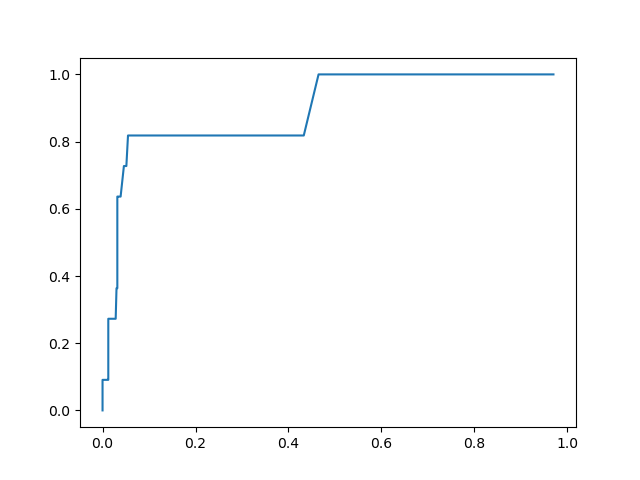
\includegraphics[width=0.7\linewidth]{./figures/roc}
    \caption{Temperature scenario. Experimental ROC curve (True Positive Rate against False Positive
        Rate) for a classifier which compares the memorability of events to a given threshold, which we vary to change the sensitivity of our detector. Measures consider 23
        manually flagged events as memorable (events added to the normal background
        as described in Section~\ref{sec:example}.)}
    \label{fig:roc}
\end{figure}

\subsection{Discussion: the subjectivity of predicates}
% todo : voir une discussion sur la notion d'influence des événements similaires/la notion de voisinage
\label{sec:discussion}
For humans, the notion of memorability and event complexity is highly subjective: the same event may appear usual for a person, while being exceptional for another. Our approach to memorability aims to reproduce this subjectivity while providing a formal canvas for memorability computations. Subjectivity is incorporated through the notion of predicates and their complexity, as they reflect the perception a human has of her surrounding environment.

\begin{figure}[!ht]
    \centering
    \begin{subfigure}{\linewidth}
        \centering
        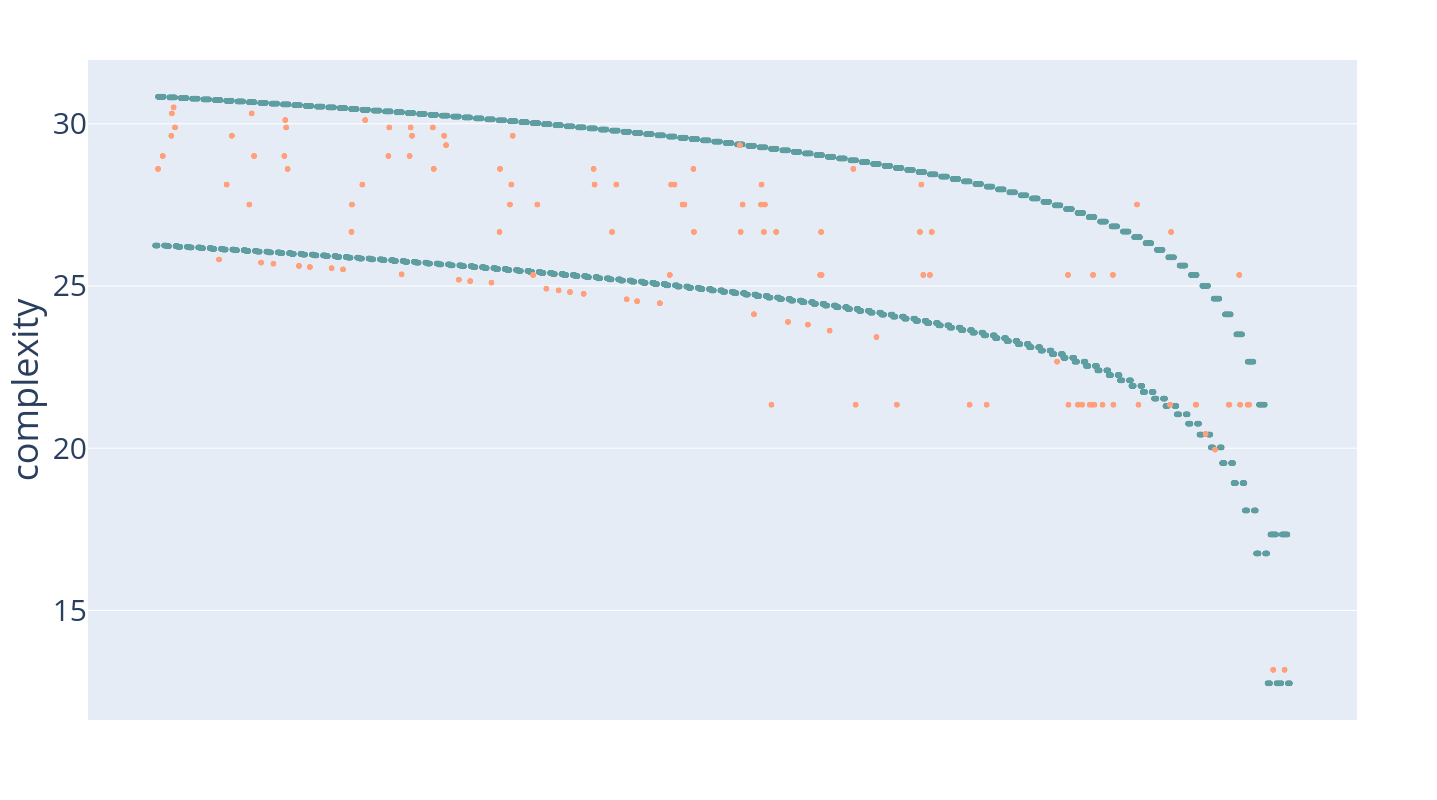
\includegraphics[width=.7\linewidth]{figures/preds_1.png}
        \caption{}
        \label{fig:pred_1}
    \end{subfigure}
    \begin{subfigure}{\linewidth}
        \centering
        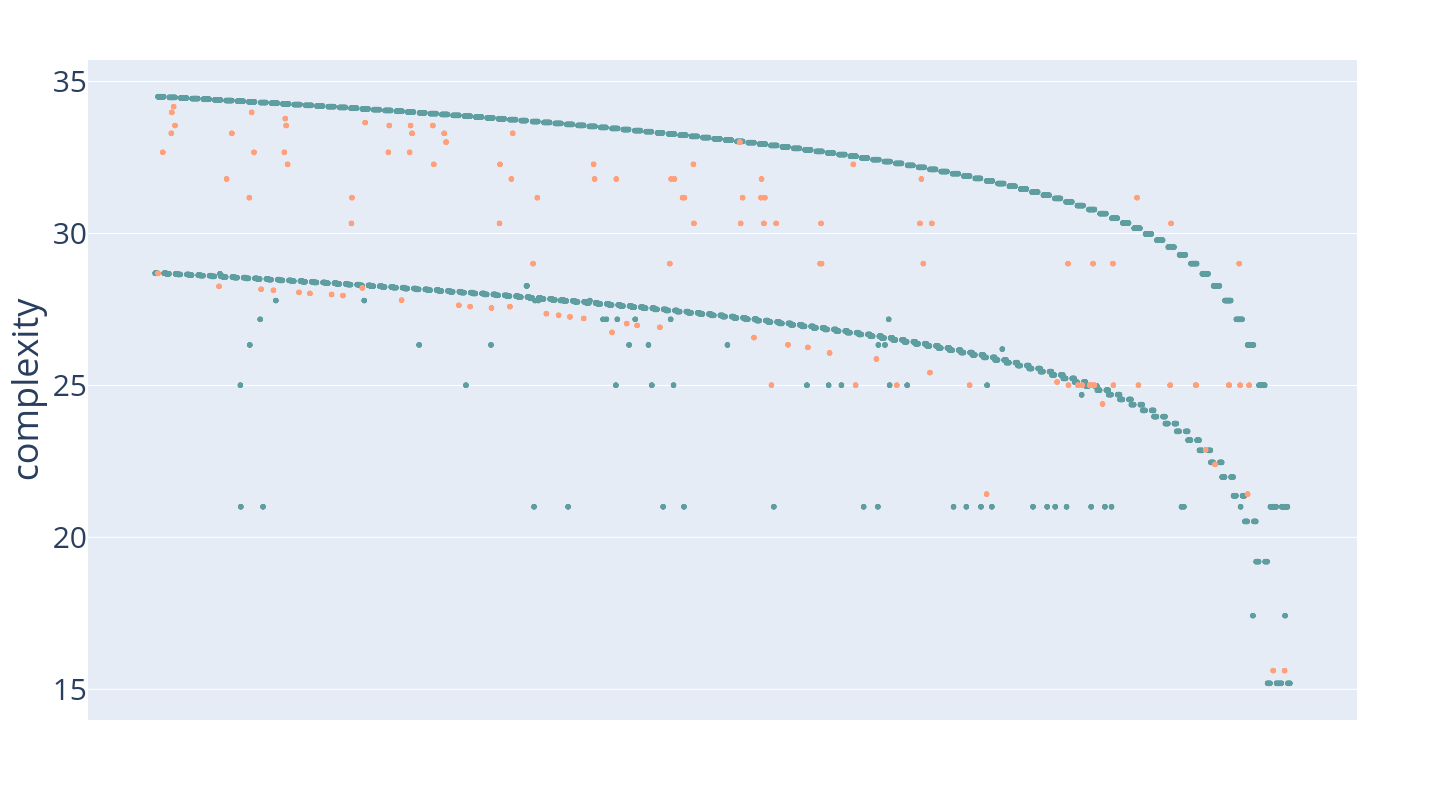
\includegraphics[width=.7\linewidth]{figures/preds_2.png}
        \caption{}
        \label{fig:pred_2}
    \end{subfigure}
    \begin{subfigure}{\linewidth}
        \centering
        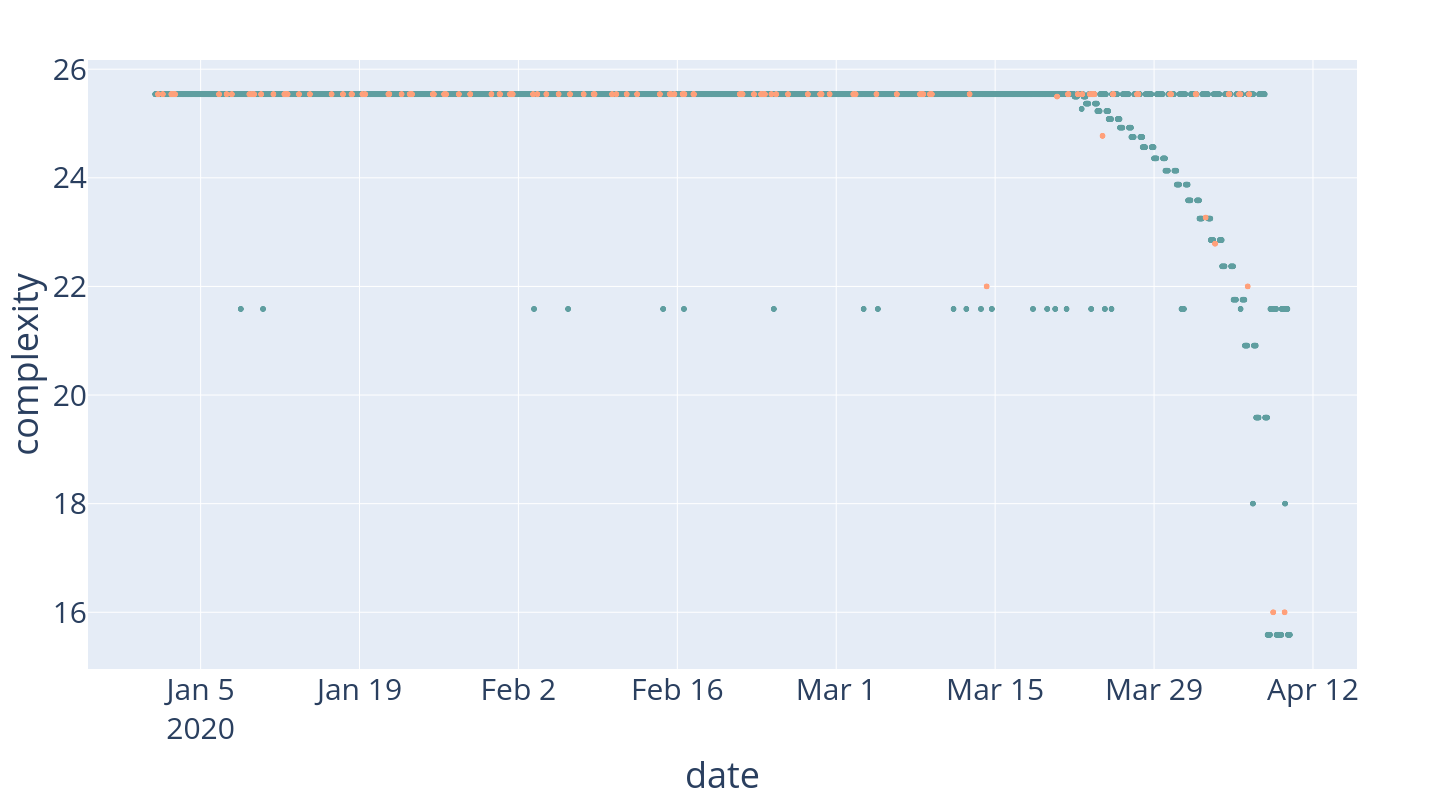
\includegraphics[width=.7\linewidth]{figures/preds_3.png}
        \caption{}
        \label{fig:pred_3}
    \end{subfigure}
    \caption{TV scenario, variation. The same memory of events, analyzed through three different sets of predicates. Light events are in blue, TV events in salmon. Figure. \ref{fig:pred_1} uses only time-related predicates (days and hours ago), while Figure. \ref{fig:pred_2} adds label predicates alongside with "dark" and day/night predicates. Figure \ref{fig:pred_3} adds the possibility to directly select any event from the memory of size $N$, at the cost of $l(N)$ bits.}
    \label{fig:3preds}
\end{figure}

In Figure \ref{fig:3preds}, we show this subjectivity by comparing the analyses of the same base memory of events, generated using the same setup as for Example 1, using three different sets of predicates. The resulting figures show different phenomena based on the predicates available to the module. In figure \ref{fig:pred_1}, only time and labels were captured by predicates. As a result, the general trend of the curve is logarithmic, as events from $T$ days ago require $O(L(T)))$ bits of information. Two main sequences of light events appear: as some light events were recorded simultaneously as TV events, they require the additional information of their label to be retrieved. In Figure \ref{fig:pred_2}, we added predicates qualifying the light intensity, along with a day/night distinction. This added capacity isolated some light events as much simpler: they all appear as aligned green points. These events are times when the light was low during day, or high during night. As such, they are outliers, and therefore require less information to be retrieved.

Finally, Figure \ref{fig:pred_3} comes from a module which has the ability to retrieve any event from a memory of size $N$, at the expense of $O(L(N))$ bits of information. This added capacity has the immediate effect of setting a clear upper limit to the description complexity of items, since any item can be retrieved using $\L(N)$ bits (in this example, this limit is around 25 bits). While this kind of direct retrieval is trivial in computer science (one could use the memory address of any stored event), its correlation to human cognition is not obvious: can humans be considered to have this possibility of selecting any event from their entire memory, without restriction regarding their nature, their time of occurrence, their magnitude? However, this highlights an interesting phenomenon: using this direct retrieval, the module makes no distinction, complexity-wise, between events past a given threshold. In other words, there is a generic "uninteresting" category of events, among which the module makes no distinction.

In addition to the number of available predicate concepts, one might also tweak their complexity. In our example scenarios, we used only a handful of predicates, hence we chose to assign all predicate concepts the same bit description length, $\log(|\Pi|)$ (see Equation. \ref{eq:pred_cost}). When using more predicate concepts, we may instead give different costs to some of them, to take into account the complexity difference between them: for instance, the generic time concept $\texttt{year}$ would likely require less bits than a predicate $\texttt{tun}$ (an old Mayan time unit, corresponding to roughly 360 days). Similar to the selection of predicates used, the complexity assigned to each predicate concept, that is, their encoding, denotes the subjectivity of the user.

%%%%%%%%%%%%%%%%%%%%%%%%%%%%%%%%%%%%%%%%%%
\section{Related Works}
\label{sec:related}
Our work is intended to be integrated into larger-scale frameworks to monitor
and detect events in complex environments such as smart homes. Smart homes are often regarded as self-organizing systems~\cite{kramer_rigorous_2009,kounev_notion_2017}. As such, they present capacities of adaptation to new goals,
new components, new environment. A commonly framework is 
autonomic computing which minimizes users' interventions for the management of the
system~\cite{kounev_notion_2017,kephart_vision_2003}.

In situations where more data is available, we could rely
on correlation or causal inference from known relations~\cite{peters_elements_2017,fadiga_or_2021}. Relations between inference and complexity have already been studied. The
case of inference was one of the motivations for R. Solomonoff to introduce his
universal algorithmic probability~\cite{solomonoff_formal_1964} as a tool to
reach an idealized inference machine, creating the notion of complexity simultaneously
to Kolmogorov. Subsequently, notions of complexity re-emerged in causal inference:
\cite{janzing_causal_2010} found than, when a causal link exists between two random variables $A \rightarrow B$, the decomposition of the joint probability is simpler in the direct than the inverse direction: $K(P(A)) + K(P(B|A)) < K(B) + K(A|B)$.

The relation between complexity, compression and causality was used in~\cite{tatti_finding_2008} to devise the PACK algorithm. It models a dataset by using a family of decision trees where each tree describes how one variable can be expressed given the others. By choosing the model minimizing the total description length (i.e. description of the model and description of the errors), PACK compresses the dataset while finding relations between variables which can be further analyzed. More recently,~\cite{marx_causal_2018} used Minimum Description Length to determine, given a joint probability distribution over $(X,Y)$, whether $X$ causes $Y$ or $Y$ causes $X$. Their method is based on tree models and it implies that a model respecting the causal relation will be simpler to describe.


Another topic where AIT can provide original approaches is event mining in data streams.
\cite{aggarwal_outlier_2017} provides a good review of modern approaches and techniques
in the field. Some previous work can also be noted for having used AIT techniques to qualify and detect events in time series data. For instance,~\cite{batista_complexity-invariant_2011,fadlallah_weighted-permutation_2013} propose weighted permutation entropy as a proxy for complexity measures in time series data, and use it to find relations between different time series.~\cite{hu_discovering_2011} proposes a MDL approach to find the intrinsic dimensions of time series.

The philosophy of our approach can be related to the ``Isolation forests'' method~\cite{liu_isolation_2008,hariri_extended_2021}. It evaluates the isolation of data points by constructing random binary tree classifiers. On average, outlier points will require less operations to be singled out. Using the average height of leaves in the tree as a metrics, this approach succeeds in identifying outlier points without having to define a ``typical'' point. This approach can be understood in terms of complexity: each node of a binary tree classifier needs a fixed amount of information to be described (it must indicates which variable and threshold are used). So nodes that are located higher in the tree need less information to be described. As such, outliers need less information to be singled out. Compared to ours, this method is tailored for data-points living in the same metric space. By using predicates as a proxy for complexity computation, our methods is more general, as it is agnostic regarding the nature of events.

While all these works advocate in favor of a strong link between complexity and the
discovery of causes, they do not extend the notion up to the point we propose in this paper, namely using the sole complexity as a tool to express the intuitive notion of memorability, and using it for inference.

\section{Perspectives}
\label{sec:future}

The practical application of the theoretical notions of event memorability $M(e)$ and relative memorability $M(c|e)$ requires further developments. We highlight two of them which seem to us, to date, the most challenging.


First, one limitation of the current approach is the requirement of
predefined predicate concepts, from which the different filters are constructed.
As an extension, we suggest the possibility of defining such predicates dynamically.
One may analyze discriminating
dimensions of incoming data and create predicates to name these differences,
similar to the contrast operations proposed in~\cite{dessalles_conceptual_2015,
    gardenfors2004conceptual}. For instance, the predicate concept $\mathtt{hot}$
can be discovered by discriminating a recent hot day along the
temperature axis and naming the difference with the prototypical day\cite{pol_multi-level_2021}.


Second, execution time is not part of the theoretical view of complexity, it
is of prime importance for practical applications, especially when one considers
implementation into real-time systems or embedded devices. While the computation
we propose appears to be heavy, and possibly heavier as the number of allowed
predicates grows, significant time savings can be achieved by trimming the base
memory of past events deemed the most ``non memorable''. For instance, one could retain
the 100 most memorable events from the past. The difficulty with
this approach is that such operations should be done without interfering with the complexity computations of new elements: by forgetting some
past events, even uninteresting ones, one should make sure to keep track of what
made the interesting ones, interesting. Investigation of how to do so can pave
the way towards practical implementations and dynamic selection of interesting
events and help reduce the memory and computation cost of data-driven applications.


%%%%%%%%%%%%%%%%%%%%%%%%%%%%%%%%%%%%%%%%%%
\section{Conclusion}

We proposed an approach to evaluate event memorability as a difference between the expected description complexity of an event and its actual value. With our definition, something is memorable if its description requires more information than expected; or less information than expected. To formalize this notion, we used principles of minimal description exposed in Algorithmic Information Theory. By defining filter operations from predicates and successively applying these filters, we defined formal ways of describing events, whose length can then be measured to evaluate their description length. From this, memorability is defined as the absolute difference between the average complexity of similar events (representing the expected complexity) and the actual description complexity of the event.


% The ability to identify some events as memorable is useful in the current context of computing, where connected devices record many events of different characteristics, magnitudes and types. This is particularly true in complex cyber-physical systems such as smart homes. We proposed an approach to evaluate the memorability as a difference between the expected description complexity of an event and its actual value. With this definition, something is memorable if it requires much less or much more information to be described. To formalize this notion, we used the Minimum Description Length principle exposed in Algorithmic Information Theory. By defining filter operations from predicates and successively applying these filters, we defined formal ways of describing events. The length of the shortest of these descriptions can be used as a measure of description complexity. From this, we defined memorability as the absolute difference between the expected and the actual description complexity. 

We provided an implementation algorithm to compute this measure on events and showed its application in two smart home examples. These scenarios qualitatively illustrate how our measure fares in comparison with the human notion of memorability, and how this measure can be used to propose relevant hypotheses in an abductive inference process without having further knowledge of the system. We discussed the inherent subjectivity of our approach by highlighting the impact of the choice of predicates for complexity computation in a toy example. We consider extending our approach by including online learning of predicates that would make our approach coincide with the subjectivity of the system's user.

The ability to identify some events as memorable is useful in the current context of computing where connected devices record many events with heterogeneous characteristics, magnitude and types. In this context, our approach of memorability aims to bring a unifying measure to sort out some events as ``memorable''. This ability can pave the way towards memorability-based abduction or selective memory.


%%%%%%%%%%%%%%%%%%%%%%%%%%%%%%%%%%%%%%%%%%
\vspace{6pt}

%%%%%%%%%%%%%%%%%%%%%%%%%%%%%%%%%%%%%%%%%%
%% optional
%\supplementary{The following are available online at \linksupplementary{s1}, Figure S1: title, Table S1: title, Video S1: title.}

% Only for the journal Methods and Protocols:
% If you wish to submit a video article, please do so with any other supplementary material.
% \supplementary{The following are available at \linksupplementary{s1}, Figure S1: title, Table S1: title, Video S1: title. A supporting video article is available at doi: link.} 

%%%%%%%%%%%%%%%%%%%%%%%%%%%%%%%%%%%%%%%%%%
\authorcontributions{Conceptualization, É. Houzé and J-L. Dessalles; methodology, software, validation, writing--original draft, É. Houzé; supervision, writing--review and editing J-L. Dessalles, A. Diaconescu and D. Menga. All authors have read and aggreed to the submitted version of the manuscript.
}



\funding{This work is part of a PhD thesis on Explainable AI for Smart Homes conducted at EDF R\&D and Télécom Paris. It is financed by EDF R\&D and the Agence Nationale pour la Recherche Technologique (ANRT).}


\dataavailability{All code and data used for the experiments can be found at \url{https://github.com/EtienneHouze/memorability_code}. The iCasa smart home simulator from the Adele research Group, which was used to generate sensor data, can be found at: \url{http://adeleresearchgroup.github.io/iCasa/snapshot/index.html}}

% \acknowledgments{In this section you can acknowledge any support given which is not covered by the author contribution or funding sections. This may include administrative and technical support, or donations in kind (e.g., materials used for experiments).}

\conflictsofinterest{The authors declare no conflict of interest.}

%% Optional
% \sampleavailability{Samples of the compounds ... are available from the authors.}

%%%%%%%%%%%%%%%%%%%%%%%%%%%%%%%%%%%%%%%%%%
%% Only for journal Encyclopedia
%\entrylink{The Link to this entry published on the encyclopedia platform.}

%%%%%%%%%%%%%%%%%%%%%%%%%%%%%%%%%%%%%%%%%%
%% Optional
% \abbreviations{Abbreviations}{
%     The following abbreviations are used in this manuscript:\\

%     \noindent
%     \begin{tabular}{@{}ll}
%         MDPI & Multidisciplinary Digital Publishing Institute \\
%         DOAJ & Directory of open access journals              \\
%         TLA  & Three letter acronym                           \\
%         LD   & Linear dichroism
%     \end{tabular}}

%%%%%%%%%%%%%%%%%%%%%%%%%%%%%%%%%%%%%%%%%%
%% Optional
% \appendixtitles{no} % Leave argument "no" if all appendix headings stay EMPTY (then no dot is printed after "Appendix A"). If the appendix sections contain a heading then change the argument to "yes".
% \appendixstart
% \appendix
% \section{}
% \subsection{}
% The appendix is an optional section that can contain details and data supplemental to the main text---for example, explanations of experimental details that would disrupt the flow of the main text but nonetheless remain crucial to understanding and reproducing the research shown; figures of replicates for experiments of which representative data are shown in the main text can be added here if brief, or as Supplementary Data. Mathematical proofs of results not central to the paper can be added as an appendix.

% \begin{specialtable}[!h]
%     \small
%     \caption{This is a table caption. Tables should be placed in the main text near to the first time they are~cited.\label{tab2}}
%     \begin{tabular}{ccc}
%         \toprule
%         \textbf{Title 1} & \textbf{Title 2} & \textbf{Title 3} \\
%         \midrule
%         Entry 1          & Data             & Data             \\
%         Entry 2          & Data             & Data             \\
%         \bottomrule
%     \end{tabular}
% \end{specialtable}

% \section{}
% All appendix sections must be cited in the main text. In the appendices, Figures, Tables, etc. should be labeled, starting with ``A''---e.g., Figure A1, Figure A2, etc.

%%%%%%%%%%%%%%%%%%%%%%%%%%%%%%%%%%%%%%%%%%
\end{paracol}
%%%%%%%%%%%%%%%%%%%%%%%%%%%%%%%%%%%%%%%%%%
% To add notes in main text, please use \endnote{} and un-comment the codes below.
%\begin{adjustwidth}{-5.0cm}{0cm}
%\printendnotes[custom]
%\end{adjustwidth}
%%%%%%%%%%%%%%%%%%%%%%%%%%%%%%%%%%%%%%%%%%
\reftitle{References}

% Please provide either the correct journal abbreviation (e.g. according to the “List of Title Word Abbreviations” http://www.issn.org/services/online-services/access-to-the-ltwa/) or the full name of the journal.
% Citations and References in Supplementary files are permitted provided that they also appear in the reference list here. 

%=====================================
% References, variant A: external bibliography
%=====================================
\externalbibliography{yes}
\bibliography{biblio}

%=====================================
% References, variant B: internal bibliography
%=====================================
% \begin{thebibliography}{999}
%     % Reference 1
%     \bibitem[Author1(year)]{ref-journal}
%     Author~1, T. The title of the cited article. {\em Journal Abbreviation} {\bf 2008}, {\em 10}, 142--149.
%     % Reference 2
%     \bibitem[Author2(year)]{ref-book1}
%     Author~2, L. The title of the cited contribution. In {\em The Book Title}; Editor1, F., Editor2, A., Eds.; Publishing House: City, Country, 2007; pp. 32--58.
%     % Reference 3
%     \bibitem[Author3(year)]{ref-book2}
%     Author 1, A.; Author 2, B. \textit{Book Title}, 3rd ed.; Publisher: Publisher Location, Country, 2008; pp. 154--196.
%     % Reference 4
%     \bibitem[Author4(year)]{ref-unpublish}
%     Author 1, A.B.; Author 2, C. Title of Unpublished Work. \textit{Abbreviated Journal Name} stage of publication (under review; accepted; in~press).
%     % Reference 5
%     \bibitem[Author5(year)]{ref-communication}
%     Author 1, A.B. (University, City, State, Country); Author 2, C. (Institute, City, State, Country). Personal communication, 2012.
%     % Reference 6
%     \bibitem[Author6(year)]{ref-proceeding}
%     Author 1, A.B.; Author 2, C.D.; Author 3, E.F. Title of Presentation. In Title of the Collected Work (if available), Proceedings of the Name of the Conference, Location of Conference, Country, Date of Conference; Editor 1, Editor 2, Eds. (if available); Publisher: City, Country, Year (if available); Abstract Number (optional), Pagination (optional).
%     % Reference 7
%     \bibitem[Author7(year)]{ref-thesis}
%     Author 1, A.B. Title of Thesis. Level of Thesis, Degree-Granting University, Location of University, Date of Completion.
%     % Reference 8
%     \bibitem[Author8(year)]{ref-url}
%     Title of Site. Available online: URL (accessed on Day Month Year).
% \end{thebibliography}

% If authors have biography, please use the format below
%\section*{Short Biography of Authors}
%\bio
%{\raisebox{-0.35cm}{\includegraphics[width=3.5cm,height=5.3cm,clip,keepaspectratio]{Definitions/author1.pdf}}}
%{\textbf{Firstname Lastname} Biography of first author}
%
%\bio
%{\raisebox{-0.35cm}{\includegraphics[width=3.5cm,height=5.3cm,clip,keepaspectratio]{Definitions/author2.jpg}}}
%{\textbf{Firstname Lastname} Biography of second author}

% The following MDPI journals use author-date citation: Admsci,  Arts, Econometrics, Economies, Genealogy, Humanities, IJFS, Jintelligence, JRFM, Languages, Laws, Literature, Religions, Risks, Social Sciences. For those journals, please follow the formatting guidelines on http://www.mdpi.com/authors/references
% To cite two works by the same author:~\citeauthor{ref-journal-1a} (\citeyear{ref-journal-1a},~\citeyear{ref-journal-1b}). This produces: Whittaker (1967, 1975)
% To cite two works by the same author with specific pages:~\citeauthor{ref-journal-3a} (\citeyear{ref-journal-3a}, p. 328;~\citeyear{ref-journal-3b}, p.475). This produces: Wong (1999, p. 328; 2000, p. 475)

%%%%%%%%%%%%%%%%%%%%%%%%%%%%%%%%%%%%%%%%%%
%% for journal Sci
%\reviewreports{\\
%Reviewer 1 comments and authors’ response\\
%Reviewer 2 comments and authors’ response\\
%Reviewer 3 comments and authors’ response
%}
%%%%%%%%%%%%%%%%%%%%%%%%%%%%%%%%%%%%%%%%%%
\end{document}

